\documentclass{article}
\usepackage{graphicx} % Required for inserting images
\usepackage{authblk} % For author affiliations
\usepackage{hyperref} % For hyperlinks
\usepackage[margin=1in]{geometry} % Standard margins
\usepackage{natbib} % For bibliography management
\usepackage{enumitem} % For customising lists
\usepackage{color}
\usepackage{amsmath}
\usepackage{float}
\usepackage{booktabs}
\usepackage{multirow} 
\usepackage{array} 
\usepackage{pdflscape}
 \usepackage{booktabs}
\usepackage{tabularray}

\newcommand\Fontvi{\fontsize{8}{8}\selectfont}

\newlist{tree}{itemize}{10}
\setlist[tree]{label=-}
\setlistdepth{10} 
\usepackage{comment}

\title{Workflow Best Practices for Infectious Disease Modelling: Multiple Data Sources, Evolving Outbreaks, and Practical Implementation}

\author[1]{Sam Abbott}
\author[2]{Xiahui Li$^\dagger$}
\author[3]{Punya Alahakoon$^\dagger$}
\author[4]{Dhorasso Junior Temfack Nguefack$^\dagger$}
\author[5]{Johannes Bracher}
\author[6]{Felix Günther}
\author[7]{Adrian Lison}
\author[8]{James Hay}
\author[9]{Oliver Eales}
\author[10]{Eben Kenah}
\author[9]{James McCaw}
\author[11]{Freya Shearer}
\author[1]{Sebastian Funk}
\author[12]{Mircea T. Sofonea}
\author[13, 14]{Pierre Nouvellet}
\author[15]{Michael J. Plank$^*$}
\author[14]{Anne Cori$^*$}
\author[16]{Anne Presanis$^*$}

\affil[1]{London School of Hygiene \& Tropical Medicine}
\affil[2]{University of St Andrews}
\affil[3]{University of Oxford}
\affil[4]{Trinity College Dublin}
\affil[5]{Karlsruhe Institute of Technology}
\affil[6]{Robert Koch Institute}
\affil[7]{Computational Evolution, ETH Zurich}
\affil[8]{Nuffield Department of Medicine, Univeristy of Oxford}
\affil[9]{School of Mathematics and Statistics, University of Melbourne}
\affil[10]{College of Public Health, Ohio State University}
\affil[11]{School of Population and Global Health, University of Melbourne}
\affil[12]{University of Montpellier}
\affil[13]{School of Life Sciences, University of Sussex}
\affil[14]{Imperial College London}
\affil[15]{School of Mathematics and Statistics, University of Canterbury}
\affil[16]{MRC Biostatistics Unit, University of Cambridge}

\renewcommand{\thefootnote}{\fnsymbol{footnote}}
\footnotetext[1]{$^\dagger$Equal contribution}
\footnotetext[2]{$^*$Equal contribution}

\date{\today}

\begin{document}

\maketitle
\newpage
\begin{abstract}
%Lead: Sam Abbott
Infectious disease modelling increasingly relies on integrating multiple data sources. Recent outbreaks have demonstrated how rapidly evolving data landscapes create both opportunities and challenges for modellers seeking to integrate diverse data streams. These settings are characterised by evolving research questions, emerging data sources, and adapting surveillance systems that require flexible analytical approaches. The infectious disease modelling community has been slow to adopt rigorous Bayesian workflow approaches, which might help mitigate these domain-specific challenges, even as these methods become increasingly formalised and widely used in other domains. This paper presents a methodological framework for integrating multiple data sources in infectious disease modelling that serves both as guidance for practitioners and as a checklist for readers evaluating modelling papers, building on general Bayesian workflow advice. We first outline an approach for characterising epidemiological data source properties through a structured checklist, then present an iterative workflow that extends established Bayesian model development approaches to the infectious disease domain, with the checklist informing decisions throughout each workflow stage. Our workflow includes defining the research question, development of directed acyclic graph (DAG) representations of process and observation models, model modularisation, inference and computation choices, model specification and validation, integration method selection, and real-world considerations. Throughout, we identify feedback loops where later decisions impact earlier choices. We provide an overview of approaches for each step as well as practical recommendations. In addition to outlining this workflow, we also give guidance on using it in evolving settings, such as outbreaks, and on good reporting practices. To demonstrate this workflow, we use schematic case studies of estimating transmission intensity with examples of how practitioners can navigate real-world trade-offs between model complexity, computational feasibility, and inferential goals. These case studies highlight how different data types can provide complementary information but may also impact other workflow choices. Our suggested framework emphasises parsimony, interpretability, and model criticism. By establishing systematic workflow practices, this framework offers a foundation for improving both the quality and transparency of infectious disease modelling, particularly during rapidly evolving outbreaks where flexible, principled approaches are essential. 
\end{abstract}
\newpage

\section{Introduction}
% Lead: Sam Abbott

% Paragraph 1: Motivation and Context
Infectious disease modelling increasingly relies on integrating multiple data sources to improve parameter estimation, reduce uncertainty, and provide more robust evidence for public health decision making \citep{deangelis2018analysing}.
Recent outbreaks, including COVID-19, mpox, and Ebola have highlighted both the potential value and practical challenges of combining diverse data streams such as case reports, deaths, hospitalisations, genomic sequences, wastewater surveillance, and serological surveys \citep{knock2021key, ro2025estimating, Abbott2021-delta, Abbott2022-prevalence, Ward2024-sp,birrell2025real}.
These outbreak settings create unique pressures where novel data streams emerge rapidly, surveillance systems evolve to meet changing needs, and models must be developed under severe time constraints with limited understanding of new data sources \citep{mccaw2023role}.
Single data sources often provide limited or biased information about key epidemiological parameters, whilst multiple sources can offer complementary perspectives that improve model accuracy and reliability or conflicting perspectives leading to flawed understanding \citep{lison2024generative, sherratt2021exploring}.
Additionally, in some cases, some parameters are only identifiable by combining data sources that together indirectly inform latent parameters, which are not directly observed \citep{deangelis2018analysing}.
However, practitioners face complex methodological choices about how to combine these, potentially conflicting, data streams effectively.

% Paragraph 2: Current Approaches
Current approaches to multi-source integration broadly fall into two categories: pipeline methods that fit separate models to individual data sources before combining estimates, and joint modelling approaches that simultaneously fit all data sources within a unified statistical framework \citep{deangelis2018analysing, russell2024combined}.
Pipeline approaches offer computational efficiency and modular development, but may propagate errors and fail to capture dependencies between data sources \citep{lison2024generative, Ward2024-sp}.
Joint modelling can provide more principled uncertainty quantification and better parameter identifiability, but often requires substantial computational resources and model complexity \citep{russell2024combined, lison2024generative}.
Recent empirical evidence supports the finding that joint approaches usually outperform stepwise methods for these reasons \citep{lison2024generative}.
Beyond these choices, practitioners face numerous challenges, including: detecting and resolving conflicts between data sources; combining data sources with different spatial or temporal resolutions; validating models when different data streams suggest different dynamics; and navigating branching decision paths where integration choices impose model structure constraints \citep{deangelis2018analysing, nicholson2022interoperability}.
Fitting challenges, such as computational intractability, parameter non-identifiability, and the need to approximate ideal model structures for practical inference, further complicate implementation \citep{corbella2022inferring, Ward2024-sp}.
These integration and fitting considerations can impact model design, yet their implications are rarely made explicit in published analyses.
Many complex multi-source models lack transparent reporting of workflow decisions, validation procedures, and code availability, creating barriers to evaluation and reproduction \citep{Ward2024-sp, Fyles2024-qz, Abbott2021-delta, Abbott2022-prevalence}.
The infectious disease modelling community has not widely adopted rigorous Bayesian workflow practices that emphasise iterative model development, systematic model criticism, and principled uncertainty quantification \citep{gelman2020bayesian, nicholson2022interoperability}.
While some recent work has partially implemented workflow elements, such as \citet{bouman2024bayesian} who explore modelling choices through simulation, these efforts lack structured guidance and omit key workflow components like prior predictive checks and systematic model criticism.
Existing guidance for practitioners is fragmented across methodological literature, with limited practical guidance for navigating these interconnected choices systematically \citep{nicholson2022interoperability, deangelis2018analysing}.

% Paragraph 3: Paper scope and contribution
This paper provides a framework for integrating multiple data sources in infectious disease modelling that serves both as guidance for practitioners and as a checklist for readers evaluating modelling papers, with practical implementation as the primary focus. 
Our approach builds on established Bayesian workflows \citep{gelman2020bayesian}, encouraging iterative model building with principled uncertainty quantification. We advocate for Bayesian thinking throughout the model development process, including model specification, model criticism, and predictive checks, regardless of whether the final implementation uses Bayesian fitting methods. 
We first outline an approach for characterising epidemiological data source properties through a structured checklist, then present an iterative workflow that extends established Bayesian model development approaches to the infectious disease domain, with the checklist informing decisions throughout each workflow stage. 
Our workflow includes defining the research question, development of directed acyclic graph (DAG) representations of process (related to or affecting transmission of the pathogen between hosts) and observation models, integration method selection, with explicit consideration of data conflicts and uncertainty quantification, inference and computation choices, and real-world considerations. Throughout, we identify feedback loops where later decisions impact earlier choices. 
We provide an overview of approaches for each step as well as practical guidelines for integration choices, validation strategies, and conflict resolution between data sources. 
As well as outlining this workflow, we also provide guidance for using it in evolving settings such as outbreaks and on good reporting practices.
Finally, we use four case studies centred on reproduction number estimation to demonstrate this workflow, progressing in complexity from a single-source baseline, through integrating similar data sources, to more complex examples with data of different types and scales. 
These case studies demonstrate broader principles applicable across infectious disease modelling contexts. 
By focusing on this common estimation task, we provide practitioners with a concrete foundation for adopting rigorous workflow practices that can then be extended to more complex modelling challenges.

\section{Data Sources and Characteristics} \label{sec:datareview}
% Lead: Punya Alahakoon

There is an increasing number of data sources being used for infectious disease surveillance and modelling, including case notifications, hospitalisations, viral load measurements from clinical samples, and wastewater samples. While each of these data sources offers unique advantages, such as timeliness, population coverage, and direct information on some quantities, they also come with distinct limitations, including reporting delays,  measurement noise, or lack of representativeness. There is currently no standardised approach to assess and compare these data sources in terms of their strengths and weaknesses, hindering our ability to compare, integrate, and prioritise data streams effectively. 

The WHO guidelines for integrated surveillance of respiratory pathogens with pandemic potential emphasise the importance of standardised, multi-purpose surveillance systems that also support public health responses and modelling \citep{world2024implementing}. Inspired by these, we propose six overarching characteristics with which to evaluate different data sources in a common framework (Figure \ref{data_characteristics}).  These characteristics are: (1) \textit{metadata}  that encapsulates foundational information about each data stream; (2) the \textit{scope} of a data source, i.e. its representative breadth and epidemiological relevance; (3) \textit{resolution} that describes the granularity and level of detail captured by a data source; (4) \textit{data quality} that encompasses the reliability, accuracy and completeness of the measurements within a data stream; (5) \textit{data utility} that refers to the practical applicability of a data source in informing epidemiological metrics and supporting public-health decision making; and (6)\textit{ practical considerations} that addresses the feasibility of using a data stream in modelling and surveillance contexts. We define additional potential criteria for each of these characteristics in the Supplementary Materials. 

We propose that these six characteristics be used as a checklist to guide the systematic assessment of a data stream's strengths and weaknesses. While the precise structure, relevance, and sub-attributes of each component may vary depending on the specific surveillance and modelling objectives, the key objective of this checklist is to promote structured, transparent thinking. We suggest first assessing our checklist within your collaboration or team,  and then modifying it to better align with your own research question. Once happy with the checklist, review each dataset available to you in turn, ideally independently and collate the responses. We then suggest summarising these responses, as demonstrated in our case study, and referring back to them through the remainder of the workflow.


\begin{figure}[H] 
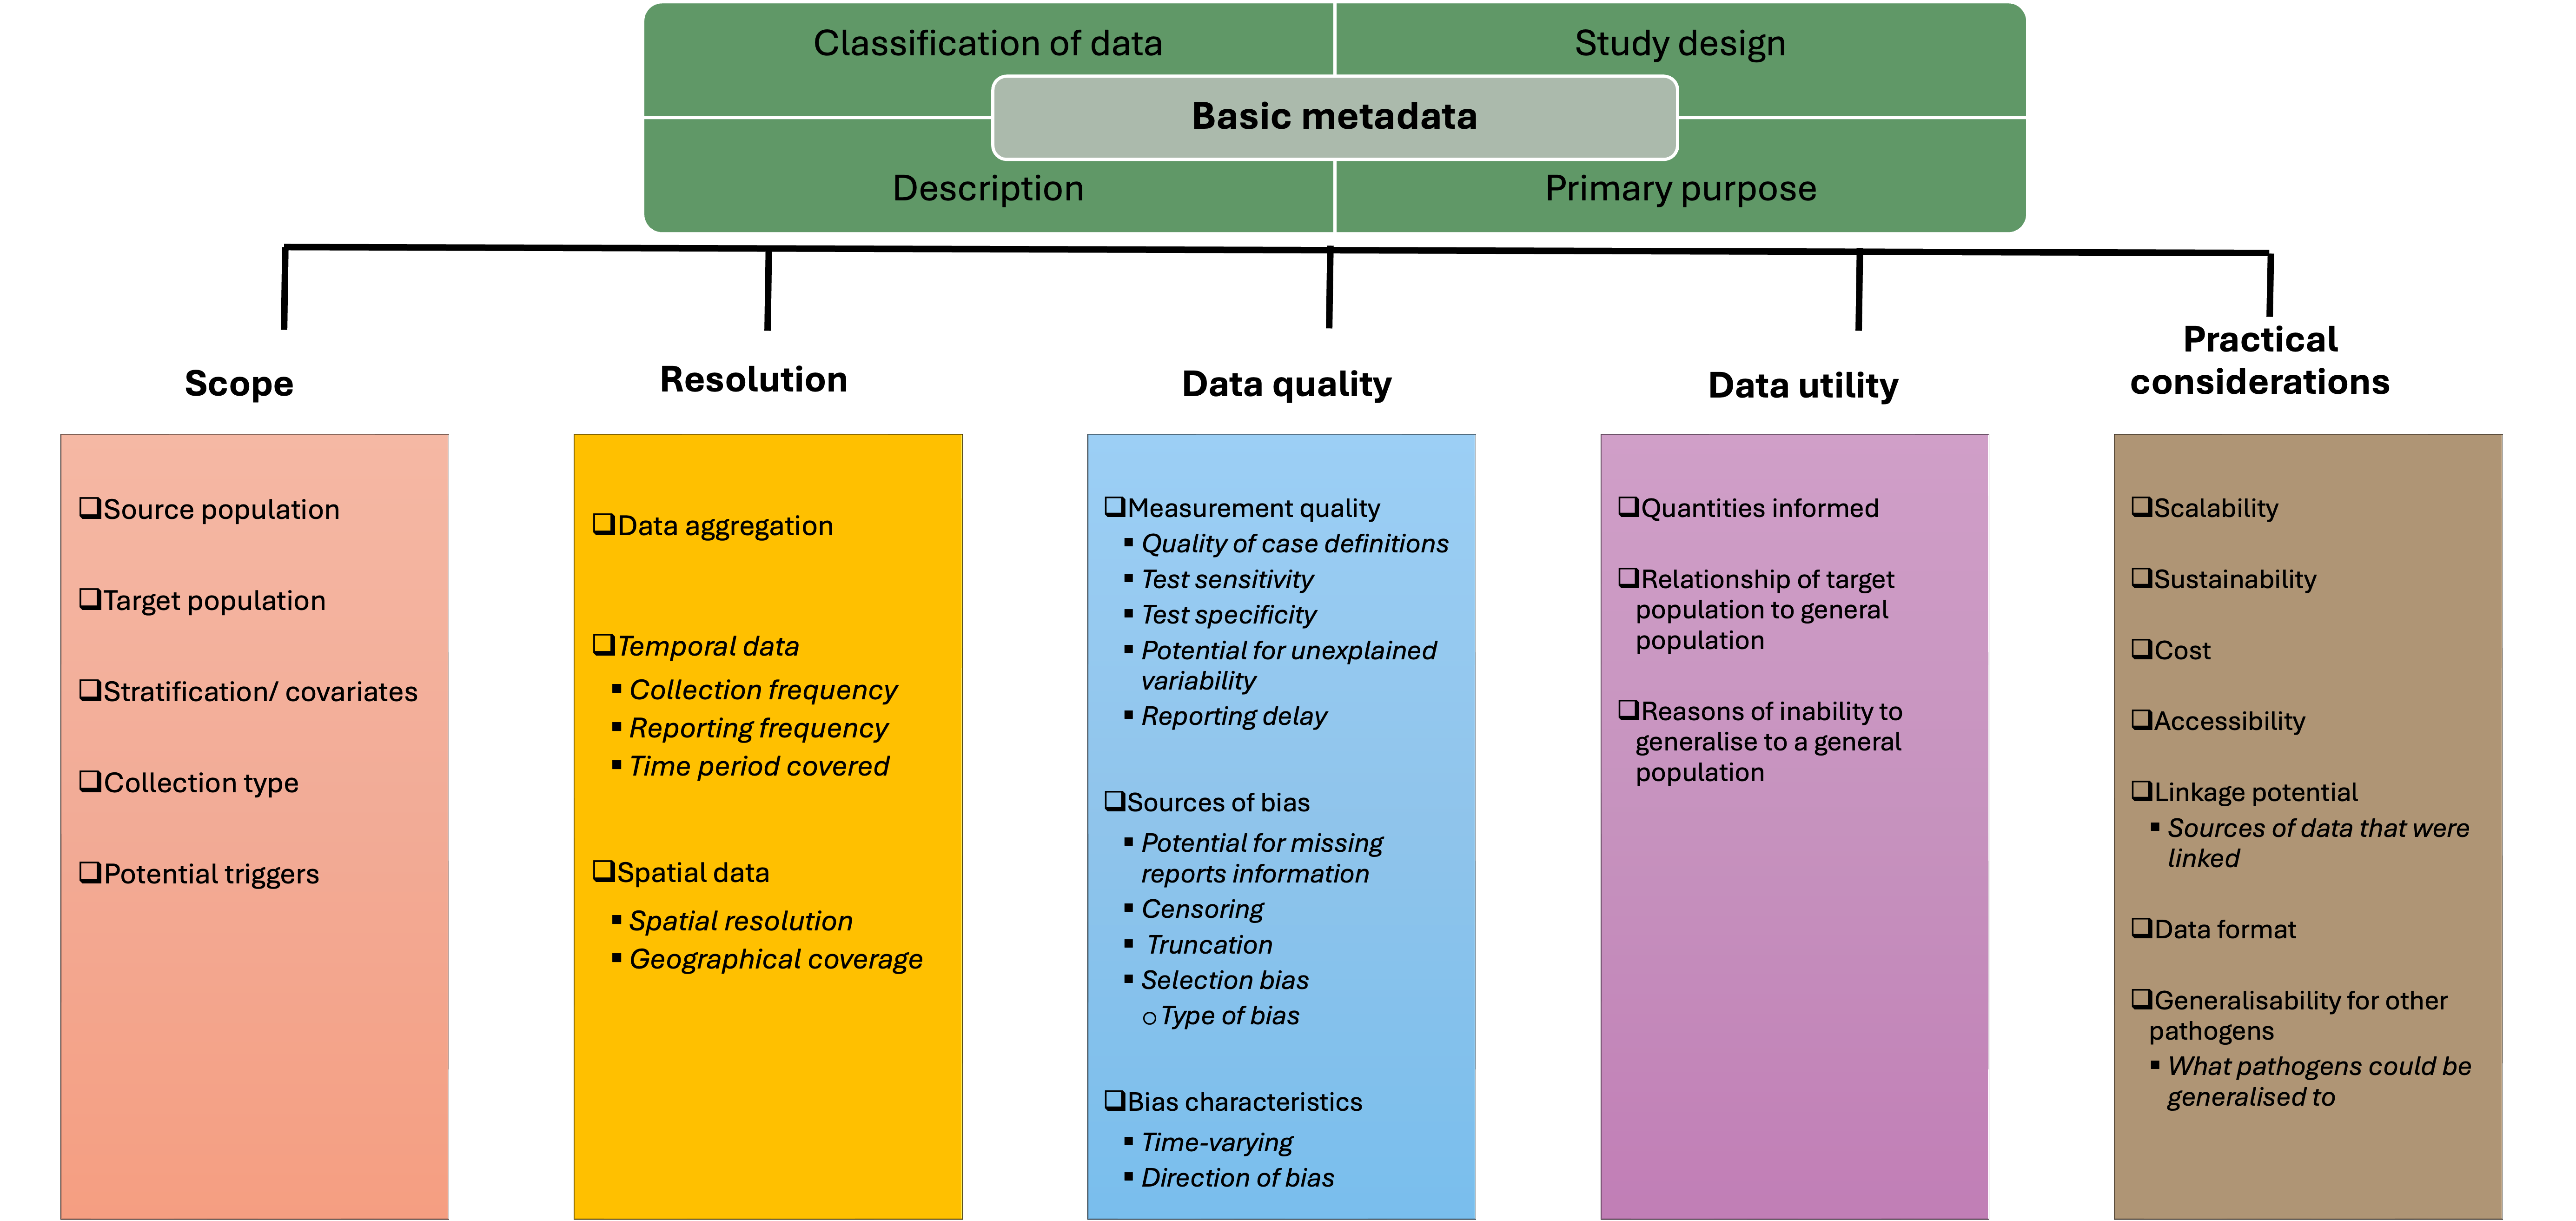
\includegraphics[width=1\linewidth]{figures/data_characteristics_2.png}
\centering
\caption{The proposed checklist for characterising a data stream used in infectious disease surveillance and modelling. The six core characteristics---metadata, scope, resolution, data quality, data utility and practical considerations---are illustrated alongside representative attributes that can be used to assess the strengths and limitations of each data source. }
\label{data_characteristics}
\end{figure}


\section{Workflow}
\label{sec:workflow}
% Lead: Sam Abbott

We recommend following a structured, iterative workflow for multi-data source modelling (Figure~\ref{fig:workflow}). Our suggested workflow extends established Bayesian workflow principles \citep{gelman2020bayesian} for  the specific challenges of multi-source infectious disease modelling.
We advocate this approach because it makes modelling choices transparent, assumptions explicit, and provides principled tools for assessing model adequacy regardless of whether final inference is Bayesian or frequentist.
The workflow should be implemented through multiple iterations, starting with high-level considerations and becoming more detailed with each pass, as some steps require later workflow components (e.g., posterior prediction requires inference and computation choices).

Begin with \textbf{decision making}: clearly define your research question and target estimands (e.g., time-varying reproduction number, overdispersion parameters).
Next, we suggest using \textbf{directed acyclic graphs (DAG)}  to define your model structure. However, we depart from standard approaches in that we suggest decoupling the definition of the \textbf{process} and \textbf{observation} models.
Here, the \textbf{process model DAG} represents the underlying epidemiological process, i.e. the transmission and related processes.
A key part of this workflow is iterating on this representation as understanding develops, i.e. during an outbreak.
The next step is to make use of the data source characterisation from the last section to \textbf{select available data sources} for your process model, such as incidence time series, genomic data, contact tracing, viral load measurements, and serological surveys based on those identified in the previous section.
Data sources should be selected based on their expected contributions to the research question.
For each data source, develop an \textbf{observation DAG} linking the underlying process to observed data through measurement models and reporting mechanisms.
Different data sources may also impact your \textbf{process DAG} assumptions, such as whether you can aggregate your representation of the process from individual-level to population-level.

Once you have developed your \textbf{process} and \textbf{observation DAGs}, \textbf{modularise your joint model} into separate sub-models for each data source, and make \textbf{inference and computation choices}, i.e. select an inference method based on the model structure, and theoretical and practical considerations for each modular model.
The next step is \textbf{Implementation considerations}, ideally following software development best practices in a probabilistic programming language.
Now you can apply \textbf{model specification and validation} to each module independently, including prior specification, parameter identifiability assessment, and prior and posterior predictive checks.
After validating individual modules, you then face key decisions on \textbf{data integration choices}: \textbf{``What to combine?''} and \textbf{``How to combine?''}.

If combining multiple sources is not beneficial or feasible, you can proceed to the combination of estimates, e.g. where multiple models are used to estimate the effective reproduction number from different data sources, and so these estimates can be ensembled.
If integration is warranted, select a \textbf{data integration} method and return to \textbf{inference and computation choices} for the newly combined models.

Throughout this workflow, there is the potential for feedback loops between steps so that model development is rarely a single forward pass (see Figure~\ref{fig:workflow}). 
Data characteristics can alter process DAG structure: individual-level data requires different representations than population-level data. 
Inference and computation constraints may require approximating or restructuring the process DAG.
Identifiability issues discovered during model specification may require simplifying either the process model or observation models. 
Practical constraints shape integration choices in multiple ways. 
Teams using incompatible programming languages may necessitate modular rather than joint approaches. 
Similarly, computational constraints may favour approximate over exact joint approaches or ensembling appraoches.
Alternatively, they can suggest refining the underlying model DAGs.
Integration complexity itself may require simplifying observation models to maintain computational feasibility. 
Conflicts between data sources during integration often reveal model misspecification, requiring revision of earlier assumptions.

In the following sections, we will discuss each of these steps in more detail and provide resources for further learning.

\begin{landscape}
\begin{figure}[htbp]
    \centering
    \includegraphics[width=\textwidth]{figures/restructured_workflow.drawio.pdf}
    \caption{\textbf{Recommended workflow for integrating multiple data sources in infectious disease modelling.} Key feedback loops from downstream parts of the workflow that impact earlier choices are represented with dashed arrows and boxes.}
    \label{fig:workflow}
\end{figure}
\end{landscape}


\subsection{Research Question and Target Estimands}

Determining the research question shapes the entire modelling workflow, from data source selection through integration choices to validation strategies.
Start by engaging with policymakers and/or stakeholders to understand which epidemiological parameters matter for their decisions: some need simple short-term admissions forecasts for hospital planning, others require transmission dynamics understanding for intervention design \citep{marshall2024when}.
Often, multiple outcomes are desired that require balancing trade-offs: short-term forecasts for operational planning alongside effective reproduction number ($R_t$) estimates for public communication and interpretability.
The aim is to translate policy needs into specific target estimands by understanding how parameters inform decisions \citep{nicholson2022interoperability, gip-2024-ru}.
For example, policymakers might need to know if transmission is increasing rather than precise values, or whether superspreading drives transmission, to choose between population-wide versus targeted interventions.
Try to define the scope explicitly, including what the analysis cannot address: a national $R_t$ estimate cannot easily reveal local outbreak dynamics, aggregate case data cannot identify transmission chains, and surveillance may not be able to detect mild infections.
These limitations shape stakeholder expectations and prevent misuse of results.
Research questions evolve throughout outbreaks as understanding improves and policy needs shift.
Early outbreak questions often focus on growth rates and severity using limited case data.
As surveillance expands, questions might shift, for example, to variant dynamics requiring genomic integration, then to population immunity needing serological data.

\subsection{Process DAG Development} \label{sec:process}

Directed acyclic graphs (DAGs) represent causal relationships through nodes  (variables) and directed edges (causal influences), making assumptions explicit and testable \citep{digitale2022tutorial}. 
This formalism helps identify confounders, mediators, and colliders that affect parameter estimation from observational data.
We recommend using Process DAGs for structuring transmission models because they separate what drives epidemics (processes related to or affecting transmission between hosts) from how we observe them.  
This separation enables modular model development where process components can be reused across different surveillance contexts \citep{nicholson2022interoperability}.
Some comment elements of process DAGs might be population structure, contact patterns, infection progression, and immunity dynamics \citep{deangelis2018analysing}. 
Your aim when constructing a process DAG  is to translate your research questions into formal causal structures that can be evaluated, communicated, and refined.
Rather than starting from scratch, we recommend aiming to adapt established epidemiological models for similar pathogens or transmission routes, modifying components as outbreak-specific data emerges \citep{gelman2020bayesian}.
Model development can begin simply and add complexity, or start comprehensive and simplify to essential components \citep{gelman2020bayesian}.
Generally, we recommend starting with a simple representation of core transmission dynamics, then iteratively refining as understanding improves or as needed by other parts of the workflow.
Early outbreak DAGs might represent homogeneous mixing, while later versions could incorporate age structure, spatial heterogeneity, or variant dynamics.
 Key biological mechanisms shape Process DAG structure. 
 For example, incubation periods create latent nodes between susceptible and infectious nodes, generation time distributions determine edges from infectious to newly infected individuals, and waning immunity adds transitions from recovered back to susceptible nodes.
 These structural choices directly affect transmission dynamics and parameter identifiability (Section~\ref{sec:spec-validate}). 

\subsection{Data Source Selection}

Now that you have a process DAG and target estimands, it is time to select data sources  from your data review using their characteristics (Section~\ref{sec:datareview}) and by identifying which epidemiological quantities each data source measures. 
For example, cases reflect infection incidence with reporting delays and ascertainment bias, hospitalisations capture severe outcomes with admission thresholds, and wastewater indicates population-level pathogen shedding independent of healthcare-seeking behaviour.
In principle, integrating multiple data sources should enhance the identifiability and precision of parameter estimates \citep{deangelis2018analysing, lison2024generative, russell2024combined, birrell2025real}. In practice, however, data integration may pose challenges. 
These include inconsistencies due to unaccounted biases \citep{presanis2013conflict,knock2021key, Ward2024-sp, corbella2022inferring}; computational complexity \citep{corbella2022inferring}; and real-time pressures during an outbreak emergency \citep{mccaw2023role}.
We therefore recommend starting with minimum data requirements for target estimands and then expanding systematically.
Evaluate complementarity by examining whether sources provide independent signals or reinforce the same information.
For example, wastewater can potentially provide early warning of outbreaks, while clinical surveillance provides individual-level severity data.
Identify redundancy where multiple sources inform the same parameter, which might improve precision, consistent with meta-analytic principles \citep{deangelis2018analysing,borenstein2021introduction}, at the cost of model complexity.

Prioritise data sources based on expected information gain relative to implementation cost.
Value-of-information methods \citep{jackson2019value,heath2024value} can formally guide whether additional data would meaningfully improve precision.
However, for complex models especially, identifiability may only become evident after fitting an initial version.

\subsection{Observation DAG Construction} \label{sec:observation}

Observation DAGs map how latent epidemiological processes generate observed data, with complexity shaped by target estimands and available data sources \citep{deangelis2018analysing}.
Build these DAGs by working backwards from measured values through all intermediate steps: symptom onset, healthcare seeking, testing, laboratory processing, and reporting for clinical surveillance; viral shedding, sewage networks, and quantification for wastewater.
Each step introduces delays, biases, or missing data mechanisms that affect inference.
Treat observation components as modular and replaceable: initial Poisson noise models can become negative binomial, simple delays can incorporate weekly patterns \citep{gelman2020bayesian}.
This flexibility reduces initial specification burden whilst enabling systematic refinement.
As for the process DAG, we recommend starting simply for each observation DAG and iteratively refining it to add complexity as required by later stages of the workflow and the research question.
Estimating population-level transmission requires simpler observation models than understanding variant-specific dynamics or age-stratified patterns.
Individual-level data enables different observation models compared to aggregated reports.
It is usually important to model reporting and other delays explicitly as they create temporal misalignment between transmission events, disease sequelae and observations \citep{seaman2022nowcasting}.
Distinguish between missing data mechanisms since random missingness and systematic under-ascertainment require different handling \citep{sherratt2021exploring}.
Account for time-varying observation probabilities from testing capacity, healthcare seeking or surveillance intensity changes.
Account for hierarchical structure and population heterogeneity whenever demographic subgroups are present in the data or required by the research question.
Multiple observation DAGs for the same underlying process enable validation by checking whether different data streams imply consistent transmission dynamics when properly integrated.

\subsection{Refine the model DAGs}

After mapping data sources and constructing your observations DAGs, revisit your process and observations DAGs to ensure alignment between what you want to model and what your data can support.
This step of the workflow aims to create a single joint DAG composed of your process and observations DAGs.
Data availability can drive both increases and decreases in model complexity.
Contact tracing data with identified transmission pairs enables shifting from population-level compartmental models to individual-based representations that capture heterogeneous mixing patterns.
Conversely, discovering that surveillance only provides aggregate counts may require collapsing a planned age-structured model into simpler compartments.
Strong prior information can sometimes compensate for data limitations, providing a further source of evidence.
For example, well-informed priors about transmission parameters from previous outbreaks might support maintaining a complex transmission model even when current data is limited and detailed knowledge about age-specific contact patterns from prior studies could support maintaining age structure, even with only total case counts.
Note that assuming fixed parameter values, common in mechanistic modelling literature, is effectively placing infinitely strong priors and should be avoided where possible in favour of appropriately uncertain prior distributions.
Temporal resolution affects what variation can be identified rather than what can be modelled: you can always build a daily-scale model, but weekly surveillance data will usually inform weekly or longer-term patterns, not daily fluctuations.
Additional DAG iteration typically occurs at key workflow stages, such as during model specification when identifiability issues emerge, during validation when misalignment between model structure and data patterns is exposed, during data integration, or due to practical or theoretical considerations related to model fitting (Figure~\ref{fig:workflow}) \citep{corbella2022inferring}.
Each iteration should address specific problems rather than making arbitrary changes.
Document why changes were made, preserving the rationale for future model extensions when better data or more domain knowledge becomes available, or when computational methods improve.
It may be the case that you are unable to use domain knowledge or reasoning to produce a single valid DAG and instead have several candidates for either or both the process and observations DAGs. 
This can often be the case when several independent teams are working on a similar problem but can also occur when mechanisms are not well-known or the data-generating process is poorly reported.
If this is the case, proceed through the remainder of the workflow with each of these candidates, comparing them in \ref{sec:spec-validate} and potentially integrating them in \ref{sec:integration}.

\subsection{Modularise Your DAGs} \label{sec:modularise}

After selecting data sources and developing and iterating on your DAGs, decompose your proposed model into modular sub-models.
Each sub-model should be as simple as possible, ideally including the process DAG and a single observation DAG, and therefore depend on a single data source.
This may mean making additional simplifying assumptions which will be relaxed during the data integration step.

We start with simple sub-models as this makes it easier to diagnose issues such as poor fit, model misspecification or convergence issues more easily.
Add complexity incrementally, only as far as needed.
This modularisation facilitates detection of inconsistencies or conflicts between data sources \citep{presanis2013conflict,manderson2023combining} and offers computational advantages over joint modelling \citep{deangelis2018analysing,goudie2019joining,gelman2020bayesian,nicholson2022interoperability}.

Apply the following workflow stages (Inference and Computation Choices, Implementation Considerations, Model Specification and Validation) to each module independently.
After validating individual modules, proceed to Data Integration Choices (Section \ref{sec:integration}) to determine how to combine them.
The integrated model may then require additional cycles through the workflow.

\subsection{Inference and Computation Choices}\label{sec:fitting}
% Lead: Xiahui and Dhorasso with support from Sam Abbott

Inference for infectious disease models involves estimating parameters $\theta$ from observed data $Y$.
 These data often arise from a probabilistic model with a likelihood function $P(Y |
  \theta)$ that links parameters to data through transmission dynamics (process DAG, Section \ref{sec:process}) and observation mechanisms (observation DAG, Section \ref{sec:observation}).
Bayesian inference, our recommended approach, updates prior beliefs $P(\theta)$ to obtain posterior distributions $P(\theta | Y) \propto P(Y|\theta) P(\theta)$, providing principled uncertainty quantification regardless of fitting method.
Inference requires balancing model complexity, computational feasibility, likelihood tractability, and available expertise.
We structure inference and computation decisions through four stages: model complexity, selecting inference methods, implementation, and diagnostics (Figure \ref{fig:fitting}). 
These choices create feedback loops within the workflow where computational constraints may require approximating or restructuring earlier DAG specifications.
This section provides an overview of these considerations.

\begin{figure}[htbp]
    \centering
    \includegraphics[width=\textwidth]{figures/restructured_fitting_workflow.drawio.pdf}
    \caption{\textbf{Inference and computation choices workflow for integrating multiple data sources in infectious disease modelling.} The workflow contains four interconnected components: Model Complexity Assessment (7.1) evaluates dimensionality, hierarchical structure, likelihood tractability, and computational constraints; Inference Method Selection (7.2) chooses between likelihood-free approaches and likelihood-based methods; Implementation Considerations (7.3) address software choices and compatibility requirements; and Diagnostics (7.4) involve convergence checks, sensitivity analysis, and computational trade-offs. The interconnected arrows indicate that these components inform each other iteratively, allowing researchers to optimize the balance between model complexity, computational feasibility, and inferential accuracy when integrating multiple data sources. The workflow includes key feedback mechanisms: inference and computation constraints may require approximating or restructuring the process DAG, leading back to stage 2 Process DAG Development. }
    \label{fig:fitting}
\end{figure}

\subsubsection{Model Complexity Assessment}

Before determining the inference approach, it is important to assess the complexity of the model.
Parameter dimensionality and structure are key to method selection as low-dimensional problems with fewer than 10 parameters require different approaches than problems with hundreds or thousands of parameters (see ``Handles high-dim. params.?'' in Table \ref{tab:methods_comparison}).
Similarly, strongly correlated parameters, discrete parameter spaces, or mixed continuous-discrete problems each impact which methods can be used or how they are implemented.
You should also consider the number of latent states such as unobserved infection times, individual-level disease states, or spatially varying transmission rates.
When there are many latent states relative to observed data, computational feasibility becomes a constraint that rules out certain approaches.
The tractability of the likelihood determines which methods can be applied.
Key questions include whether the likelihood $P(Y | \theta)$ can be written analytically, evaluated numerically at reasonable cost, or differentiated with respect to parameters.
Models with stochastic differential equations or discrete event processes often lack tractable likelihoods.
This rules out methods that require likelihood evaluation or gradients.

\subsubsection{Inference Method Selection}

Numerous inference methods and algorithmic variants exist within each broad class of approach, each with distinct computational characteristics and practical trade-offs.
Selecting an appropriate method involves balancing considerations of computational efficiency, statistical rigour, data availability, interpretability, and model complexity.
Rather than adopting a universal approach, the choice should be tailored to the specific modelling context and inferential goals.
The following gives guidance to selecting a method, but does not cover all settings.

Gradient-based Markov Chain Monte Carlo (MCMC) approaches represent our preferred methods when applicable due to their combination of efficiency, reliability, and ease of use \citep{gilks1995markov, lekone2006statistical}.
MCMC methods generate samples from the posterior distribution by constructing a Markov chain that converges to the target distribution, providing a flexible framework for Bayesian inference when analytical solutions are unavailable.
Hamiltonian Monte Carlo (HMC) leverages gradient information for efficient MCMC exploration of differentiable likelihoods, with its adaptive variant No-U-Turn Sampler (NUTS) representing our default recommendation for models with continuous parameters, or where discrete parameters can be marginalised out \citep{duane1987hybrid, hoffman2014no, andrade2020evaluation}.
When implementing gradient-based methods, the automatic differentiation method can have a substantial impact: forward-mode differentiation suits models with few parameters (typically fewer than 10), whilst reverse-mode differentiation scales better for high-dimensional parameter spaces.
Practitioners should test available automatic differentiation options when possible.
When full uncertainty quantification is less critical, Variational Inference (VI) approximates the posterior by optimising tractable surrogate distributions, offering fast approximation with modern variants like Pathfinder \citep{blei2017variational, chatzilena2019contemporary}.

Sampling-based approaches become necessary when gradients are unavailable.
Standard Markov Chain Monte Carlo (MCMC) methods including Metropolis-Hastings and Gibbs sampling handle discrete or mixed parameter spaces \citep{hastings1970monte, geman1984stochastic, gilks1995markov}.
For discrete parameters, consider whether marginalisation is possible before resorting to sampling, as analytical integration can significantly improve efficiency and mixing.
Parallel tempering extends these methods to multimodal posteriors by running multiple chains at different temperatures, with modern implementations available in packages like Pigeons.jl \citep{surjanovic2023pigeons}.
For models in which the latent state dimension grows over time, as in state-space models, MCMC becomes increasingly inefficient.

Sequential Monte Carlo (SMC) methods, or particle filters, offer a natural alternative in such models by approximating the filtering distribution of latent states using weighted particles. They enable online Bayesian updating as new observations arrive, making them well-suited for real-time epidemic tracking \citep{doucet2001introduction, birrell2020efficient, storvik2023sequential}. However, SMC alone is less efficient for parameter inference. Particle MCMC (PMCMC) addresses this limitation by combining SMC with MCMC to enable joint inference of states and parameters \citep{andrieu2010particle, endo2019introduction}. Key limitations of particle-based methods include particle degeneracy (where few particles carry most weight) and  memory scaling challenges with long time series. Table \ref{tab:methods_comparison} summarizes these relative strengths and limitations.
 
Approximate Bayesian inference methods provide efficient alternatives for specific model structures.
Integrated Nested Laplace Approximation (INLA) offers a computationally efficient method for approximating posterior marginals in latent Gaussian models, making it particularly effective for spatiotemporal disease models with spatial correlation structures \citep{rue2017bayesian}.
This method excels when models can be reformulated with latent Gaussian components but struggles with non-Gaussian latent structures.

Deterministic approaches focus on point estimation rather than uncertainty quantification.
Maximum Likelihood Estimation (MLE) provides point estimates for model parameters, particularly useful for simple models requiring only parameter estimates rather than full uncertainty quantification, or for prototyping \citep{myung2003tutorial, baltazar2024maximum}.
Profile likelihood methods extend MLE by examining the likelihood surface for individual parameters whilst optimising over others, providing confidence intervals without full posterior sampling \citep{tonsing2018profile, plank2024structured}.

Likelihood-free approaches are methods of last resort due to their computational demands and limited diagnostic capabilities.
These simulation-based methods bypass likelihood evaluation entirely, instead using model simulations to approximate the posterior distribution.
Approximate Bayesian Computation (ABC) approximates the posterior distribution by accepting parameter values that generate simulated data close to the observed data under a predefined distance metric, whilst synthetic likelihood methods approximate the likelihood by assuming Gaussian distributions for summary statistics \citep{beaumont2002approximate, wood2010statistical, price2018bayesian}.

\begin{landscape}
\begin{table}[ht]
\renewcommand{\arraystretch}{1.2}
\centering
\caption{\textbf{Comparison of Likelihood-Based and Likelihood-Free Fitting Methods.} 
This table focuses on foundational algorithms. More recent methodological advancements that build upon these classical approaches are discussed in Section 4.9 of the main text. ``PPL'' stands for Probabilistic Programming Languages. For this review, PPL examples include Stan, PyMC, JAGS, NIMBLE, Turing.jl, etc.}
\label{tab:methods_comparison}
\small
\begin{tabular}{@{}p{3.5cm}p{1.5cm}p{1.5cm}p{1.5cm}p{1.5cm}p{1.5cm}p{1.5cm}p{1.5cm}p{1.5cm}@{}}
\toprule
\multirow{2}{*}{\textbf{Feature}} & \multicolumn{6}{c}{\textbf{Likelihood-Based}} & \multicolumn{2}{c}{\textbf{Likelihood-Free}} \\
\cmidrule(lr){2-7} \cmidrule(lr){8-9}
 & MLE & MCMC & SMC & PMCMC & INLA & VI & ABC & BSL \\
\midrule
\textbf{Theoretical Considerations} & & & & & & & & \\
\midrule
Requires likelihood? & Yes & Yes & Yes & Yes & Yes & Yes & No & No \\
Handles high-dim. params.? & Poor & Moderate & Moderate & Moderate & Good & Good & Moderate & Moderate \\
Convergence guarantees & Asymptotic & Asymptotic & Asymptotic & Asymptotic & Approx. & Approx. & Approx. & Approx. \\
Distributional flexibility & Low & High & High & High & Medium & Medium & High & Medium \\
Approximation error & Exact (asymp.) & Exact (asymp.) & Particle-based & Exact (asymp.) & Deterministic & Variational & Simulation & Simulation \\
\midrule
\textbf{Practical Considerations} & & & & & & & & \\
\midrule
Computational cost & Low & High & Med--High & Very high & Low & Low--Med & High & High \\
Scalability (big data) & Good & Poor & Moderate & Poor & Good & Good & Moderate & Moderate \\
Example software & PPL & PPL & LibBi & POMP, NIMBLE & R-INLA & PPL & abctools, EasyABC, ELFI & ELFI \\
Tuning required? & Minimal & Step size, priors & Resampling & Complex & Minimal & ELBO opt. & Sum. stats., distance, threshold & Sum. stats. \\
Capable of real-time inference? & Yes & No & Yes & No & Yes & Yes & No & No \\
Parallelization potential & 
High & 
Limited, chain-level, GPU possible but hard & 
High, particle-level, GPU possible & 
Limited, particle-level, GPU possible for simple models & 
Low, matrix operation hard to parallelise & 
Medium, gradient parallelisation; GPU possible & 
High, simulations parallelisable; GPU possible & 
Medium, GPU possible \\
Diagnostics & Likelihood ratio & $\hat{R}$, ESS, Trace& ESS & $\hat{R}$, ESS,Trace & Residuals & ELBO, PPC & Acc.~rate, PPC & Acc.~rate, PPC \\
Best use case & Simple models & General Bayesian inference & Real-time inference & State-space models & Latent Gaussian models & Fast approximation & Intractable likelihood & Intractable likelihood + summary stats \\
\bottomrule
\end{tabular}
\end{table}
\end{landscape}

% Table \ref{tab:methods_comparison} provides detailed comparison across multiple criteria to support these decisions.

\paragraph{Hybrid and Nested Approaches}

Modern probabilistic programming languages enable sophisticated combinations of inference methods.
INLA approximations can be nested within NUTS, using efficient spatial approximations while sampling other parameters.
Languages like Turing.jl support mixed samplers, applying HMC to continuous parameters whilst using Gibbs for discrete components \citet{fjelde2025turing}.
SMC methods can incorporate HMC kernels for parameter moves, leveraging particle filtering for states and gradient-based sampling for parameters \citet{buchholz2021adaptive, devlin2024no, rosato2024enhanced}.
These hybrid approaches capitalise on the strengths of multiple methods.

When complex methods fail to initialise properly within prior bounds, simpler methods can provide starting values for more sophisticated approaches.
Variational Inference often proves effective for initialisation due to its speed and robustness, whilst MLE can provide reasonable point estimates.
However, initialisation difficulties may indicate unrealistic prior specifications, suggesting model validation should be revisited before proceeding with complex inference.

\subsubsection{Implementation considerations}

We recommend balancing computational cost against inferential quality when implementing your chosen inference method, considering both model complexity and available computational resources (Table \ref{tab:methods_comparison}) \citep{funk2020choices}.
We recommend prioritising methods with automatic tuning to reduce implementation burden and improve reliability.
HMC and NUTS require minimal manual intervention through automatic step size adaptation and mass matrix estimation, making them accessible to practitioners with limited MCMC experience.
Standard MCMC and particle methods demand careful tuning of proposals, particle counts, and resampling thresholds through pilot runs.
ABC approaches require the most expertise for selecting summary statistics, distance metrics, and tolerance thresholds.
INLA and VI may require upfront model reformulation to fit their frameworks.

Parallelisation can determine whether methods can scale to population-level inference or handle real-time analysis during outbreaks.
Methods differ substantially in their parallelisation capabilities (Table \ref{tab:methods_comparison}).
MCMC methods face inherent parallelisation challenges due to their sequential chain structure.
Multi-chain parallelisation provides the primary scaling mechanism.
Parallel tempering exploits multi-core architectures through temperature-parallel chains \citep{surjanovic2023pigeons}.
Some implementations support within-chain parallelisation for gradient calculations (Stan and Turing.jl) or matrix operations (GPU acceleration).
VI scales well through mini-batch parallelisation and routinely uses GPU acceleration for large datasets \citep{hoffman2013stochastic, Abbott2021-delta}.
Sequential and particle methods excel at parallelisation through particle-level parallelism.
Modern GPUs enable thousands of particles to be processed simultaneously.
Memory requirements scale with particle count \citep{henriksen2012parallel}.
Approximate methods show mixed potential.
INLA has limited opportunities due to sequential matrix operations, though some implementations exploit parallel linear algebra libraries.
Nested approximations can parallelise across spatial or temporal components when model structure permits.
Likelihood-free methods provide parallelisation opportunities for rejection-based ABC.
Rejection ABC parallelises trivially across CPU clusters and GPU architectures.
ABC-MCMC retains the sequential constraints of MCMC methods.
Memory requirements can become substantial for large simulated datasets \citep{kulkarni2022hardware}.
Deterministic approaches parallelise most effectively.
MLE is highly parallelisable across data points on both CPUs and GPUs.
Profile likelihood calculations naturally parallelise across parameter values.

\subsubsection{Diagnostics}

The quality and availability of diagnostic tools vary substantially across inference methods, representing a key factor in method selection (see Table \ref{tab:methods_comparison} for method-specific diagnostics).
HMC and NUTS provide the gold standard with divergence warnings, BFMI, energy plots, and traditional MCMC diagnostics like $\hat{R}$ and ESS, making them easier to use reliably, particularly for practitioners without extensive computational expertise.
Standard MCMC and parallel tempering offer moderate diagnostic capabilities through traditional convergence statistics and trace plots, with parallel tempering adding temperature swap rates to monitor multimodal exploration.
SMC and PMCMC methods rely on particle-specific metrics including effective sample size (ESS) and weight degeneracy to track sequential performance and detect particle impoverishment. 
In contrast, Variational Inference provides only ELBO convergence monitoring (which does not guarantee accurate posterior approximation), whilst ABC methods offer minimal diagnostics through acceptance rates alone, making both heavily dependent on posterior predictive checks (PPC) for validation.
Diagnostic failures across any method indicate potential model specification issues requiring systematic validation procedures (Section \ref{sec:spec-validate}), with specific patterns like divergent transitions in NUTS suggesting posterior geometry problems requiring structural model changes.

\subsection{Model Implementation}\label{sec:implementation}

\subsubsection{Setting Up Your Implementation Environment}

For implementing your models, we recommend using a probabilistic programming language (PPL).
PPLs and their ecosystems make many tasks in model specification and validation more straightforward (Section \ref{sec:spec-validate}).
The precise choice often depends on the fitting approach selected in the subsequent section (Section \ref{sec:fitting}), and in some cases, using a PPL may not be possible.
Generally, using the same implementation approach for all model components will require the least amount of effort.

Generative PPLs where you can sample from and compute gradients for the same model specification are particularly valuable.
Turing.jl, PyMC, and NumPyro provide this capability \citep{ge2018turing,fjelde2025turing,abril2023pymc,phan2019composable}, enabling simulation-based validation approaches without separate data generators.
Stan offers the most mature diagnostic and validation tools \citep{carpenter2017stan} , but requires separate simulation code.
JAGS and NIMBLE offer flexibility for model structures that may not be well-suited to gradient-based methods \citep{plummer2003jags,valpine2017programming}.
Turing.jl is likely the most composable option \citep{ge2018turing}, which proves useful when building models from modules.
Speed is difficult to assess and is often model and context-specific, though generally Stan and NumPyro are the most efficient options when applicable \citep{carpenter2017stan,phan2019composable}.
Selecting a flexible implementation approach is important for evolving settings (Section \ref{sec:outbreak}).

Making use of standard software development practices is likely to improve all aspects of your workflow \citep{gelman2020bayesian}.
These include: unit testing to verify model components, continuous integration to catch errors early, version control to track model evolution, and comprehensive test coverage for data processing and diagnostics.

\subsubsection{Building Modular DAG Components}

Translate your modularised DAGs (Section \ref{sec:modularise}) into separate code modules.
Structure observation models as interchangeable components connecting to process models through defined interfaces (e.g., both case and wastewater modules interface through infection incidence).
Document interfaces explicitly to enable component reuse across teams.

Maintain consistent parameter naming between mathematical formulation and code when possible.
Start with minimal implementations, adding complexity only as validation confirms necessity.

\subsection{Model Specification and Validation}\label{sec:spec-validate}

Follow the systematic Bayesian workflow for model validation \citep{gelman2020bayesian}, working through structured phases that provide clear decision points and feedback loops.
Start by validating models in small subcomponents first, then explore combinations to identify integration challenges early.

\subsubsection{Prior Specification and Prior Predictive Checks}

Specify priors using domain knowledge where available through informative priors; otherwise, use weakly informative priors that regularise without dominating the likelihood.
Prior predictive checks simulate data from the prior to ensure model behaviour is epidemiologically plausible before seeing data and to detect prior-data conflict \citep{Box1980,yang2025detecting}.
These checks can reveal several issues requiring model modification: unrealistic parameter ranges may indicate the need for different priors or model constraints; implausible epidemic dynamics may suggest DAG structural changes; computational issues during simulation may indicate need for model approximations or reparameterisation.
Results of prior predictive checks may indicate a need to either: revisit prior specification, e.g. to obtain additional data sources, previous estimates or expert consultation to inform appropriate prior distributions; or return to DAG development (Sections \ref{sec:process} and \ref{sec:observation}) to simplify models, add model components, increase complexity through hierarchical structure, or implement approximations for computational tractability.

\subsubsection{Model Fitting and Computational Validation}

After resolving issues raised by prior-predictive checks, fit the model using methods from Section \ref{sec:fitting}.
Validate computational aspects, such as convergence and algorithm performance, through diagnostic checks, synthetic data simulation, and simulation-based calibration where feasible.
Using simulated scenarios to validate parameter recovery provides valuable insights into model performance \citep{bouman2024bayesian}, whilst simulation-based calibration for each submodel provides stronger validation by verifying that inference algorithms can recover true parameters from simulated data \citep{talts2018validating}.
Address computational issues systematically: simplify model structure or increase prior informativeness if convergence fails; examine submodels in detail if joint fitting proves intractable; reparameterise models if mixing is poor; plot intermediate quantities like effective reproduction numbers to identify problematic components; run on data subsets or reduce iterations to speed up iteration; check for multimodality using multiple chains or parallel tempering \citep{gelman2020bayesian}.
Remember that the goal is to make predictions or learn about epidemiological processes, not merely achieve convergence of an arbitrary model. 
If computational validation succeeds, provisionally accept the model for posterior validation.
Persistent computational issues require returning to model specification or considering alternative integration approaches (Section \ref{sec:integration}).

\subsubsection{Evaluate and Use Model}

Begin with posterior- and mixed-predictive checks \citep{rubin1984bayesianly,gelman1995bayesian} to assess whether fitted models reproduce key features across all integrated sources.
These checks form the foundation of model validation by comparing model-generated predictions against observed patterns.
Apply cross-validation strategies, particularly leave-one-out and time-aware validation, to assess predictive performance whilst avoiding conservatism due to double use of the data and respecting temporal data structure.
Examine influence of individual data points and prior specifications through sensitivity analysis.

Assess parameter identifiability by examining whether data sources provide sufficient information to uniquely estimate target parameters; joint modelling often resolves identifiability issues that plague pipeline approaches \citep{lison2024generative, russell2024combined}.
For some models, structural identifiability approaches \citep{jackson2019value,heath2024value} may be used to indicate where additional data or prior information is needed.
Implement poststratification as needed to correct for population representativeness issues.

Conflict arises when data sources and/or prior information provide inconsistent evidence on model parameters.
We detect conflict between data sources when different streams imply incompatible parameter values under the current model.
Conflicts may arise between prior assumptions and data (``prior-data conflict''), between different data sources, or even within a data source but between different units of data \citep{presanis2013conflict,yang2025detecting}.
These conflicts typically manifest as lack of identifiability (with convergence problems as a symptom) or lack of fit to one or more data sources \citep{presanis2013conflict,deangelis2018analysing}. Detection methods based on generalising cross-validatory posterior-/mixed-predictive checks to any latent node in a DAG \citep{presanis2013conflict,yang2025detecting} usually also measure the extent of conflict. We can use complementary  prior sensitivity analysis to quantify how much priors must change to accommodate observed data, revealing potential model misspecification or data quality issues \citep{Roos2015,Kallioinen2024,yang2025detecting}.

We resolve conflicts through careful consideration of unaccounted biases or overly restrictive model assumptions.
Adjust model structure as needed, including loosening prior assumptions, implementing weighting approaches for selection biases, and other bias modelling approaches \citep{deangelis2018analysing}.
This starts another cycle of the model development and criticism process.

If posterior validation reveals model inadequacies, return to DAG development to modify model structure, add complexity, or implement different approximations.

\subsubsection{Model Comparison}

When multiple plausible model specifications exist, use Leave-One-Out Cross-Validation (LOO-CV), Watanabe-Akaike Information Criterion (WAIC), Continuous Ranked Probability Score (CRPS), or other methods to compare predictive accuracy \citep{vehtari2017practical,yao2018using,gneiting2007strictly} combined with visual posterior predictive checks.
High Pareto-k values from LOO-CV identify influential observations requiring careful modelling.
For infectious disease models, consider scoring transformations such as the log when using CRPS \citep{bosse2023scoring}.
Maximise sharpness subject to calibration: models should produce statistically consistent predictions whilst minimising required uncertainty \citep{gneiting2007strictly}.
Model comparison serves as the final validation step, ensuring that chosen specifications provide optimal predictive performance whilst maintaining epidemiological interpretability.

\subsection{Data Integration Choices}\label{sec:integration}
% Lead: Anne Presanis

Decisions about data integration are inherently context-dependent, but can be guided by the decision tree in Figure \ref{fig:integration}. We recommend combining the modularised models sequentially and repeating the validation processes outlined in \ref{sec:spec-validate} for each newly combined module, repeating this process until the full model has been implemented and validated.
We further recommend using joint modelling of these modules where possible, taking advantage of Markov melding \citep{goudie2019joining} or its approximations where possible and computationally required,  and making use of cut distributions \citep{plummer2015cuts} if needed (Section \ref{sec:joint}). 
This joint modelling approach offers a coherent framework for integrating such sources simultaneously, in the spirit of Bayesian hierarchical models \citep{gelman2020bayesian}, with suitable uncertainty quantification and avoiding the definitional ambiguities that affect output-level combinations \citep{manley2024combining, brockhaus2023why}. 

Ensemble methods (Section \ref{sec:ensembling}) are valuable when joint modelling proves impossible due to computational constraints, data access limitations, or institutional boundaries between research teams.
When employing ensembles, careful attention to ensuring all models target the same estimand, resolving temporal alignment, and documenting methodological assumptions becomes essential for meaningful combination. 

When combining independent model outputs from different groups, the choice of ensembling or meta-analytic approach should align with the research objective (e.g. estimation or prediction), influencing how estimates or predictions are weighted (e.g. by precision or prediction accuracy). In contrast, when integrating sub-models, the approach will depend on whether existing sub-models have already been fitted or if the models are being developed de novo.

In addition to prior-data conflict and submodel conflict, different data sources may also conflict. These types of conflict should be assessed during the model validation and specification process, as discussed in Section \ref{sec:spec-validate} \citep{presanis2013conflict,sherratt2021exploring,yang2025detecting}, once the data integration process has been decided upon.

The following sections have additional details on integration approaches.

\subsubsection{Full joint modelling}\label{sec:joint}

A fully joint modelling approach is especially suited when there are complex dependencies between data sources \citep{corbella2022inferring}, perhaps conditional on the parameters of the underlying process model, such that identification of all parameters is compromised when some data are left out. However, joint models can be computationally intensive and challenging to fit, especially in high-dimensional or real-time settings. Care is needed to ensure complex dependencies are appropriately modelled and that observational biases, such as selection biases, are adequately accounted for in the model, to avoid conflict between data sources \citep{presanis2013conflict,corbella2022inferring}. 

\subsubsection{Markov melding} Techniques like Markov melding \citep{goudie2019joining} allow posterior samples from one sub-model to serve as a proposal distribution for the next, potentially in a sequential chain of models \citep{manderson2023combining}. Similar sequential strategies, using the posterior from one sub-model as the prior (rather than proposal) for another, have a long history \citep{west1997bayesian}, closely related to Sequential Monte Carlo algorithms \citep{doucet2001introduction} (see Section \ref{sec:fitting}).

\subsubsection{Approximations of Markov melding} While the theory and some applications of Markov melding are well-established \citep{goudie2019joining,nicholson2022interoperability,manderson2023combining}, practical implementation remains challenging. Limitations include the availability of user-friendly Bayesian software and methods for assessing sub-model compatibility and combining them \citep{yang2025detecting}. As a result, approximate methods are often used. A common approach is the one used in standard meta-analysis \citep{borenstein2021introduction} to combine previous estimates using a normal approximation. A Stage 1 point estimate, $\hat{y}_1$, and its corresponding standard error or posterior standard deviation $\hat{\sigma}^2_1$, can be incorporated in a Stage 2 model as a likelihood term, on an appropriate scale:
$$
\hat{y}_1 \sim N(\theta, \hat{\sigma}^2_1)
$$ for some parameter $\theta$ in the Stage 2 model informed by the Stage 1 estimate. This approach has been shown to be an approximation to Markov melding with ``product of experts'' pooling \citep{goudie2019joining}.

\subsubsection{Cut posteriors}

Modular approaches also support judgements of selective trust in sub-models, as indicated by the name ``modularisation'' in the first appearance of a ``cut'' posterior in the literature \citep{LiuEtAl2009}. This approach `cuts' feedback from one module to another, i.e. preventing less reliable sub-models from influencing more trusted ones while allowing the reverse, providing robustness against sub-model misspecification \citep{plummer2015cuts,carmona2022scalable,yu2023variational}. \citet{liu2025general} provide a general framework for deciding how to partition and restrict information flow between sub-models. As with Markov melding, however, practical implementation remains a challenge, since it involves a potentially computationally expensive multiple imputation approach for each MCMC sample \citep{plummer2015cuts}.

\subsubsection{Ensembling independent models}\label{sec:ensembling}

When multiple models target the same estimand, ensemble methods such as Bayesian stacking \citep{yao2018using}, model averaging \citep{hoeting1999bayesian}, or meta-analytical pooling \citep{jackson2011multivariate} can be used to combine estimates.
This is similar to comparing models as discussed in Section \ref{sec:spec-validate} .
These differ from approaches like Markov melding in that they combine independent model outputs rather than partitioning a joint model into connected sub-models.
The choice of ensemble strategy should reflect the research objective.
For prediction, weighting by out-of-sample accuracy may be appropriate; for estimation, weights might reflect precision or model credibility \citep{yao2018using}.
Ensemble methods offer practical advantages when joint modelling proves infeasible, enabling collaboration between research teams and potentially improving robustness over single models.
The European COVID-19 Forecast Hub demonstrated performance gains from simple median aggregation \citep{sherratt2021exploring}, whilst the UK's SPI-M consensus used random-effects meta-analysis to pool $R_t$ estimates from multiple academic groups \citep{manley2024combining}.

However, important limitations constrain ensemble approaches for infectious disease modelling.
When models make different assumptions about latent quantities, apparent heterogeneity may reflect definitional differences rather than true uncertainty about the estimand \citep{brockhaus2023why}.
Temporal alignment becomes particularly problematic for latent targets where the underlying definition remains ambiguous, with models using different reference points, generation time distributions, or reporting delay assumptions \citep{brockhaus2023why}.
This can lead to estimates that are less timely and/or less precise, with lower utility for decision makers than the component models \citep{manley2024combining}.
Combining outputs at the prediction level discards information about data conflicts and model disagreements that would be preserved in joint modelling approaches.
Weighted ensemble methods often show limited improvement over simple aggregation in nowcasting applications \citep{sherratt2021exploring}, partly because the black-box nature of many models obscures why predictions differ.

\begin{figure}[htbp]
    \centering
    \includegraphics[width=\textwidth]{figures/integration choices decision tree.drawio.pdf}
    \caption{\textbf{Decision tree for integration choices when integrating multiple data sources in infectious disease model inference.} The flowchart guides researchers through key decision points to select appropriate integration strategies.}
    \label{fig:integration}
\end{figure}

\section{Workflow Management}

\subsection{Outbreak Evolution and Workflow Iteration}  \label{sec:outbreak}
% Lead Sam Abbott
Two types of changes during outbreaks require revisiting this workflow.
First, new information emerges about pathogen characteristics, surveillance capabilities, and population dynamics that may necessitate updating model assumptions and data integration choices \citep{mccaw2023role}.
Second, research questions evolve as outbreak priorities shift from initial detection and characterisation towards intervention evaluation and long-term planning.
When these changes occur, practitioners should iterate through the workflow, revisiting their earlier decisions, rather than developing entirely new models.

Changes that warrant workflow iteration include: substantial new data sources becoming available (such as genomic surveillance or serological surveys); shifts in research questions that alter target estimands; and improved understanding of pathogen biology that changes process model assumptions \citep{knock2021key}.
The modular approach we advocate enables practitioners to update specific workflow components whilst preserving elements from previous iterations.
For example, observation models developed for case surveillance can often be reused when adding death reporting, whilst process models for transmission dynamics may require updating when new variants emerge.
This incremental approach reduces development time and maintains continuity across evolving outbreak contexts.

These steps are often carried out on an ad-hoc basis by teams during outbreaks but we think that a more formal approach that tracks decisions is likely to improve the quality of models produced and be ultimately less resource-intensive.
Establishing regular review points to assess whether workflow iteration is needed is likely to be beneficial with more regular reviews during acute outbreak phases.
Each iteration should document what has changed, why updates are necessary, and how new approaches build upon previous work.
Having this documentation supports both real-time decision-making and retrospective evaluation of analytical approaches.

\subsection{Reporting} \label{sec:reporting}
% Lead Sam Abbott
Complex multi-source models require clear documentation to enable evaluation and reproduction.
Without structured reporting, even well-designed workflows are challenging to assess or improve.
Reporting decisions made at each stage of the workflow is essential, including rationales for data source selection, integration method choices, model structure assumptions, and validation procedures undertaken.
Making analyses public at all stages builds trust, though confidential data requires careful management \citep{Abbott2021-delta, Abbott2022-prevalence}.

We recommend sharing code and data alongside results because it enables verification, accelerates progress, as it just as much a part of the analysis as the manuscript.
Not sharing code, sharing it on request \citep{Ward2024-sp}, or only once a paper is in a peer-reviewed journal \citep{Fyles2024-qz} , all create barriers to assessing data integration workflows.
Where barriers to transparent reporting exist, it is always better to report as much as possible.
Mathematical specifications, validation code, and synthetic examples all contribute to transparency even when data cannot be shared.
When data cannot be shared, synthetic data generation helps readers understand model behaviour \citep{Mellor2025-norovirus}.

We also recommend visual schematics of the workflow used and the model architecture. An example of this is Ward et al.'s analysis of COVID-19 hospitalisation and fatality risk, which provides useful visual communication of model relationships but would benefit from process DAGs and code availability \citep{Ward2024-sp}.

\section{Case Studies}
% Lead: Michael Plank

We demonstrate our iterative workflow through four progressive case study schematics, each building complexity whilst showing different integration choices and methodological considerations.
All case studies share a common estimand -- the time-varying reproduction number ($R_t$) -- while the final case study has the overdispersion parameter ($k$) as an additional estimand.

The progression between case studies illustrates key principles relating to the characterisation of different data sources. Case study 0 uses a single data source, reported case counts. Case study 1 combines case data with data on deaths, enabling some of the limitations of each single data source to be overcome. Case study 2 adds wastewater data as a third data source that is independent of testing patterns and biases. Case studies 0, 1 and 2 all deal with aggregated data that cannot provide information about individual variability. Case study 3 combines case count data with individual-level data on transmission pairs to enable direct overdispersion estimation without distributional assumptions.
To support these case studies, we first give an example of our suggested data review approach.

\subsection{Data Sources and Characteristics}

We designed and completed a questionnaire based on the key data characteristics we suggested (Section \ref{sec:datareview}). We first developed targeted questions aligned with each characteristic to facilitate systematic and accessible characterisation. These questions (see Supplementary Material S2) were designed to support both qualitative and quantitative evaluation across data sources. We then completed it for a range of data sources (Supplementary Material S2). Here, we focus on the data sources used in our case studies: time series of confirmed cases, deaths, wastewater surveillance data, and transmission-paired observations.

We found that data sources differed across all six characteristics, with substantial variation in responses reflecting differences in subjective interpretation, context, and experience (Figure \ref{survey_responses}, Table \ref{tab:survey_results}). For \textbf{Basic metadata}, we felt that 83\% of confirmed case collections served clinical management, while all wastewater collections served non-clinical purposes. Under \textbf{Scope}, we thought that confirmed case data usually targeted the whole population (100\%),  and wastewater datasets were split between geographic structure (40\%) and whole population (60\%). We considered both sources to have high geographic coverage (mean: 4.5 [range: 4-5] for cases; 4 [3-5] for wastewater (where 1 is low and 5 is high)). For \textbf{Resolution}, we thought that confirmed case datasets were a mix of aggregated (33\%) and individual-level data (67\%). In contrast, we saw wastewater data as entirely aggregated (100\%), though our responses diverged on stratification and reporting frequency. All authors thought that all datasets included temporal information, but that only 50\% of case datasets included spatial information data. \textbf{Data quality} assessments suggested we perceived similar test sensitivity (mean: 4 [range: 3-5] for cases; 3.8 [3-5] for wastewater), but we differed in perceived population representativeness (4.3 [3-5] for cases; 3 [1-4] for wastewater). We thought both sources informed key epidemiological quantities with varying directness and notable disagreement under \textbf{Data utility}: we were split on the role of case data for informing prevalence between directly (33\%), indirectly (33\%), or not informed (33\%), while we all saw wastewater data as indirectly informing prevalence (100\%). Under \textbf{Practical considerations}, we perceived scalability as predominantly linear for both sources (67\% for cases; 80\% for wastewater), but our perceptions of sustainability differed markedly (1 for all case datasets; 3.3 [2-5] for wastewater). Overall, we saw greater feasibility for long-term wastewater surveillance. The variation in our views highlights the importance of acknowledging context-specific practices when evaluating data sources, while demonstrating that the six core characteristics provide a systematic framework for context-sensitive assessment of their strengths and limitations.

{\Fontvi
% \usepackage{color}
% \usepackage{tabularray}
\definecolor{Shark}{rgb}{0.125,0.129,0.141}
\definecolor{Alto}{rgb}{0.827,0.827,0.827}
\begin{longtblr}[
  caption = {Categorical survey responses for confirmed time series (6 responses), wastewater (5 responses), deaths (XX responses), and transmission pairs (XX responses).},
 label = {tab:survey_results},
  entry = none,
]{
  width = \linewidth,
  colspec = {Q[129]Q[342]Q[163]Q[96]Q[65]Q[60]Q[60]},
  cell{1}{3} = {c},
  cell{1}{4} = {c},
  cell{1}{6} = {c=2}{0.12\linewidth},
  cell{2}{1} = {fg=Shark},
  cell{2}{3} = {c},
  cell{2}{4} = {c},
  cell{2}{6} = {c=2}{0.12\linewidth},
  cell{3}{3} = {c},
  cell{3}{4} = {c},
  cell{3}{6} = {c=2}{0.12\linewidth},
  cell{4}{3} = {c},
  cell{4}{4} = {c},
  cell{4}{6} = {c=2}{0.12\linewidth},
  cell{5}{3} = {c},
  cell{5}{4} = {c},
  cell{5}{6} = {c=2}{0.12\linewidth},
  cell{6}{3} = {c},
  cell{6}{4} = {c},
  cell{6}{6} = {c=2}{0.12\linewidth},
  cell{7}{3} = {c},
  cell{7}{4} = {c},
  cell{7}{6} = {c=2}{0.12\linewidth},
  cell{8}{3} = {c},
  cell{8}{4} = {c},
  cell{8}{6} = {c=2}{0.12\linewidth},
  cell{9}{3} = {c},
  cell{9}{4} = {c},
  cell{9}{6} = {c=2}{0.12\linewidth},
  cell{10}{3} = {c},
  cell{10}{4} = {c},
  cell{10}{6} = {c=2}{0.12\linewidth},
  cell{11}{3} = {c},
  cell{11}{4} = {c},
  cell{11}{6} = {c=2}{0.12\linewidth},
  cell{12}{3} = {c},
  cell{12}{4} = {c},
  cell{12}{6} = {c=2}{0.12\linewidth},
  cell{13}{3} = {c},
  cell{13}{4} = {c},
  cell{13}{6} = {c=2}{0.12\linewidth},
  cell{14}{3} = {c},
  cell{14}{4} = {c},
  cell{14}{6} = {c=2}{0.12\linewidth},
  cell{15}{3} = {c},
  cell{15}{4} = {c},
  cell{15}{6} = {c=2}{0.12\linewidth},
  cell{16}{3} = {c},
  cell{16}{4} = {c},
  cell{16}{6} = {c=2}{0.12\linewidth},
  cell{17}{3} = {c},
  cell{17}{4} = {c},
  cell{17}{6} = {c=2}{0.12\linewidth},
  cell{18}{3} = {c},
  cell{18}{4} = {c},
  cell{18}{6} = {c=2}{0.12\linewidth},
  cell{19}{3} = {c},
  cell{19}{4} = {c},
  cell{19}{6} = {c=2}{0.12\linewidth},
  cell{20}{1} = {fg=Shark},
  cell{20}{3} = {c},
  cell{20}{4} = {c},
  cell{20}{6} = {c=2}{0.12\linewidth},
  cell{21}{3} = {c},
  cell{21}{4} = {c},
  cell{21}{6} = {c=2}{0.12\linewidth},
  cell{22}{3} = {c},
  cell{22}{4} = {c},
  cell{22}{6} = {c=2}{0.12\linewidth},
  cell{23}{3} = {c},
  cell{23}{4} = {c},
  cell{23}{6} = {c=2}{0.12\linewidth},
  cell{24}{3} = {c},
  cell{24}{4} = {c},
  cell{24}{6} = {c=2}{0.12\linewidth},
  cell{25}{3} = {c},
  cell{25}{4} = {c},
  cell{25}{6} = {c=2}{0.12\linewidth},
  cell{26}{3} = {c},
  cell{26}{4} = {c},
  cell{26}{6} = {c=2}{0.12\linewidth},
  cell{27}{3} = {c},
  cell{27}{4} = {c},
  cell{27}{6} = {c=2}{0.12\linewidth},
  cell{28}{3} = {c},
  cell{28}{4} = {c},
  cell{28}{6} = {c=2}{0.12\linewidth},
  cell{29}{3} = {c},
  cell{29}{4} = {c},
  cell{29}{6} = {c=2}{0.12\linewidth},
  cell{30}{3} = {c},
  cell{30}{4} = {c},
  cell{30}{6} = {c=2}{0.12\linewidth},
  cell{31}{3} = {c},
  cell{31}{4} = {c},
  cell{31}{6} = {c=2}{0.12\linewidth},
  cell{32}{3} = {c},
  cell{32}{4} = {c},
  cell{32}{6} = {c=2}{0.12\linewidth},
  cell{33}{3} = {c},
  cell{33}{4} = {c},
  cell{33}{6} = {c=2}{0.12\linewidth},
  cell{34}{3} = {c},
  cell{34}{4} = {c},
  cell{34}{6} = {c=2}{0.12\linewidth},
  cell{35}{3} = {c},
  cell{35}{4} = {c},
  cell{35}{6} = {c=2}{0.12\linewidth},
  cell{36}{3} = {c},
  cell{36}{4} = {c},
  cell{36}{6} = {c=2}{0.12\linewidth},
  cell{37}{3} = {c},
  cell{37}{4} = {c},
  cell{37}{6} = {c=2}{0.12\linewidth},
  cell{38}{3} = {c},
  cell{38}{4} = {c},
  cell{38}{6} = {c=2}{0.12\linewidth},
  cell{39}{3} = {c},
  cell{39}{4} = {c},
  cell{39}{6} = {c=2}{0.12\linewidth},
  cell{40}{3} = {c},
  cell{40}{4} = {c},
  cell{40}{6} = {c=2}{0.12\linewidth},
  cell{41}{3} = {c},
  cell{41}{4} = {c},
  cell{41}{6} = {c=2}{0.12\linewidth},
  cell{42}{3} = {c},
  cell{42}{4} = {c},
  cell{42}{6} = {c=2}{0.12\linewidth},
  cell{43}{3} = {c},
  cell{43}{4} = {c},
  cell{43}{6} = {c=2}{0.12\linewidth},
  cell{44}{3} = {c},
  cell{44}{4} = {c},
  cell{44}{6} = {c=2}{0.12\linewidth},
  cell{45}{3} = {c},
  cell{45}{4} = {c},
  cell{45}{6} = {c=2}{0.12\linewidth},
  cell{46}{3} = {c},
  cell{46}{4} = {c},
  cell{46}{6} = {c=2}{0.12\linewidth},
  cell{47}{3} = {c},
  cell{47}{4} = {c},
  cell{47}{6} = {c=2}{0.12\linewidth},
  cell{48}{3} = {c},
  cell{48}{4} = {c},
  cell{48}{6} = {c=2}{0.12\linewidth},
  cell{49}{3} = {c},
  cell{49}{4} = {c},
  cell{49}{6} = {c=2}{0.12\linewidth},
  cell{50}{3} = {c},
  cell{50}{4} = {c},
  cell{50}{6} = {c=2}{0.12\linewidth},
  cell{51}{3} = {c},
  cell{51}{4} = {c},
  cell{51}{6} = {c=2}{0.12\linewidth},
  cell{52}{3} = {c},
  cell{52}{4} = {c},
  cell{52}{6} = {c=2}{0.12\linewidth},
  cell{53}{3} = {c},
  cell{53}{4} = {c},
  cell{53}{6} = {c=2}{0.12\linewidth},
  cell{54}{3} = {c},
  cell{54}{4} = {c},
  cell{54}{6} = {c=2}{0.12\linewidth},
  cell{55}{3} = {c},
  cell{55}{4} = {c},
  cell{55}{6} = {c=2}{0.12\linewidth},
  cell{56}{3} = {c},
  cell{56}{4} = {c},
  cell{56}{6} = {c=2}{0.12\linewidth},
  cell{57}{3} = {c},
  cell{57}{4} = {c},
  cell{57}{6} = {c=2}{0.12\linewidth},
  cell{58}{3} = {c},
  cell{58}{4} = {c},
  cell{58}{6} = {c=2}{0.12\linewidth},
  cell{59}{3} = {c},
  cell{59}{4} = {c},
  cell{59}{6} = {c=2}{0.12\linewidth},
  cell{60}{3} = {c},
  cell{60}{4} = {c},
  cell{60}{6} = {c=2}{0.12\linewidth},
  cell{61}{3} = {c},
  cell{61}{4} = {c},
  cell{61}{6} = {c=2}{0.12\linewidth},
  cell{62}{3} = {c},
  cell{62}{4} = {c},
  cell{62}{6} = {c=2}{0.12\linewidth},
  cell{63}{3} = {c},
  cell{63}{4} = {c},
  cell{63}{6} = {c=2}{0.12\linewidth},
  cell{64}{3} = {c},
  cell{64}{4} = {c},
  cell{64}{6} = {c=2}{0.12\linewidth},
  cell{65}{3} = {c},
  cell{65}{4} = {c},
  cell{65}{6} = {c=2}{0.12\linewidth},
  cell{66}{3} = {c},
  cell{66}{4} = {c},
  cell{66}{6} = {c=2}{0.12\linewidth},
  cell{67}{3} = {c},
  cell{67}{4} = {c},
  cell{67}{6} = {c=2}{0.12\linewidth},
  cell{68}{3} = {c},
  cell{68}{4} = {c},
  cell{68}{6} = {c=2}{0.12\linewidth},
  cell{69}{3} = {c},
  cell{69}{4} = {c},
  cell{69}{6} = {c=2}{0.12\linewidth},
  cell{70}{3} = {c},
  cell{70}{4} = {c},
  cell{70}{6} = {c=2}{0.12\linewidth},
  cell{71}{3} = {c},
  cell{71}{4} = {c},
  cell{71}{6} = {c=2}{0.12\linewidth},
  hline{1,73} = {-}{0.08em},
  hline{2,8,20,43,68,72} = {-}{},
  hline{3-7,9-19,21-42,44-67,69-71} = {2-7}{Alto},
}
\textbf{Core characteristic} & \textbf{Sub-characteristic} & {\textbf{Confirmed cases time series}\\N = 6\textit{\textsuperscript{1}}} & {\textbf{Wastewater}\\N = 5\textit{\textsuperscript{1}}} & {\textbf{Deaths}\\N=?~} & {\textbf{Transmission paires~}\\N=?\textbf{}} & \\
{\textbf{Basic}\\\textbf{~meta-data}} & \textbf{Study design} &  &  &  &  & \\
 & ~~~~Routine surveillance & 6 (100\%) & 3 (60\%) &  &  & \\
 & ~~~~Sentinel surveillance & 0 (0\%) & 2 (40\%) &  &  & \\
 & \textbf{Primary purpose} &  &  &  &  & \\
 & ~~~~Clinical management & 5 (83\%) & 0 (0\%) &  &  & \\
 & ~~~Other & 1(17\%) & 5 (10\%) &  &  & \\
\textbf{\textbf{Scope}} & \textbf{Target population} &  &  &  &  & \\
 & ~~~~Geographic structure & 0 (0\%) & 2 (40\%) &  &  & \\
 & ~~~~Whole population & 6 (100\%) & 3 (60\%) &  &  & \\
 & \textbf{Stratification/covariates (except spatial-temporal see Resolution section)} &  &  &  &  & \\
 & ~~~~Demographic & 1 (17\%) & 0 (0\%) &  &  & \\
 & ~~~~Demographic, Clinical & 3 (50\%) & 0 (0\%) &  &  & \\
 & ~~~~None & 2 (33\%) & 5 (100\%) &  &  & \\
 & \textbf{Collection type} &  &  &  &  & \\
 & ~~~~Routine & 6 (100\%) & 5 (100\%) &  &  & \\
 & \textbf{If triggered, potential triggers} &  &  &  &  & \\
 & ~~~~New variant/pathogen detected & 1 (100\%) & 0 (NA\%) &  &  & \\
 & ~~~~Unknown & 5 & 5 &  &  & \\
\textbf{Resolution} & \textbf{Data aggregation} &  &  &  &  & \\
 & ~~~~Aggregated & 2 (33\%) & 5 (100\%) &  &  & \\
 & ~~~~Individual & 4 (67\%) & 0 (0\%) &  &  & \\
 & \textbf{Temporal data} &  &  &  &  & \\
 & ~~~~Yes & 6 (100\%) & 5 (100\%) &  &  & \\
 & \textbf{Collection frequency} &  &  &  &  & \\
 & ~~~~Continuously & 1 (17\%) & 1 (20\%) &  &  & \\
 & ~~~~Daily & 4 (67\%) & 0 (0\%) &  &  & \\
 & ~~~~Multiple times a week & 0 (0\%) & 3 (60\%) &  &  & \\
 & ~~~~Weekly & 1 (17\%) & 1 (20\%) &  &  & \\
 & \textbf{Reporting frequency} &  &  &  &  & \\
 & ~~~~Daily & 3 (50\%) & 0 (0\%) &  &  & \\
 & ~~~~Multiple times a week & 0 (0\%) & 2 (40\%) &  &  & \\
 & ~~~~Weekly & 3 (50\%) & 3 (60\%) &  &  & \\
 & \textbf{Time period covered} &  &  &  &  & \\
 & ~~~~all the time & 0 (0\%) & 1 (20\%) &  &  & \\
 & ~~~~Continuous & 6 (100\%) & 3 (60\%) &  &  & \\
 & ~~~~Endemic & 0 (0\%) & 1 (20\%) &  &  & \\
 & \textbf{Spatial data} & 3 (50\%) & 5 (100\%) &  &  & \\
 & \textbf{Spatial resolution} &  &  &  &  & \\
 & ~~~~Local & 1 (17\%) & 5 (100\%) &  &  & \\
 & ~~~~National & 2 (33\%) & 0 (0\%) &  &  & \\
 & ~~~~Regional & 3 (50\%) & 0 (0\%) &  &  & \\
\textbf{Data utility} & \textbf{Quantities informed [Basic reproduction number]} &  &  &  &  & \\
 & ~~~~Direct & 0 (0\%) & 1 (20\%) &  &  & \\
 & ~~~~Indirect & 5 (83\%) & 0 (0\%) &  &  & \\
 & ~~~~Not informed & 1 (17\%) & 4 (80\%) &  &  & \\
 & Qu\textbf{antities informed [Time-varying reproduction number]} &  &  &  &  & \\
 & ~~~~Direct & 4 (67\%) & 1 (20\%) &  &  & \\
 & ~~~~Indirect & 2 (33\%) & 4 (80\%) &  &  & \\
 & \textbf{Quantities informed [Time-varying / basic reproduction number ratio]} &  &  &  &  & \\
 & ~~~~Direct & 0 (0\%) & 1 (20\%) &  &  & \\
 & ~~~~Indirect & 5 (83\%) & 0 (0\%) &  &  & \\
 & ~~~~Not informed & 1 (17\%) & 4 (80\%) &  &  & \\
 & \textbf{Quantities informed [Incidence]} &  &  &  &  & \\
 & ~~~~Direct & 3 (50\%) & 0 (0\%) &  &  & \\
 & ~~~~Indirect & 3 (50\%) & 4 (80\%) &  &  & \\
 & ~~~~Not informed & 0 (0\%) & 1 (20\%) &  &  & \\
 & \textbf{Quantities informed [Prevalence]} &  &  &  &  & \\
 & ~~~~Direct & 2 (33\%) & 0 (0\%) &  &  & \\
 & ~~~~Indirect & 2 (33\%) & 5 (100\%) &  &  & \\
 & ~~~~Not informed & 2 (33\%) & 0 (0\%) &  &  & \\
 & \textbf{Quantities informed [Heterogeneity in transmission (e.g. superspreading)]} &  &  &  &  & \\
 & ~~~~Indirect & 4 (67\%) & 0 (0\%) &  &  & \\
 & ~~~~Not informed & 2 (33\%) & 5 (100\%) &  &  & \\
 & \textbf{Quantities informed [Drivers of transmission]} &  &  &  &  & \\
 & ~~~~Indirect & 3 (50\%) & 0 (0\%) &  &  & \\
 & ~~~~Not informed & 3 (50\%) & 5 (100\%) &  &  & \\
\textbf{\textbf{Practical considerations}} & \textbf{Scalability} &  &  &  &  & \\
 & ~~~~Independent & 0 (0\%) & 4 (80\%) &  &  & \\
 & ~~~~Linearly & 4 (67\%) & 0 (0\%) &  &  & \\
 & ~~~~Sub-exponentially & 2 (33\%) & 1 (20\%) &  &  & \\
 & \textit{\textsuperscript{1}}~n (\%) &  &  &  &  & 
\end{longtblr}
}

%
\begin{figure}[H] 
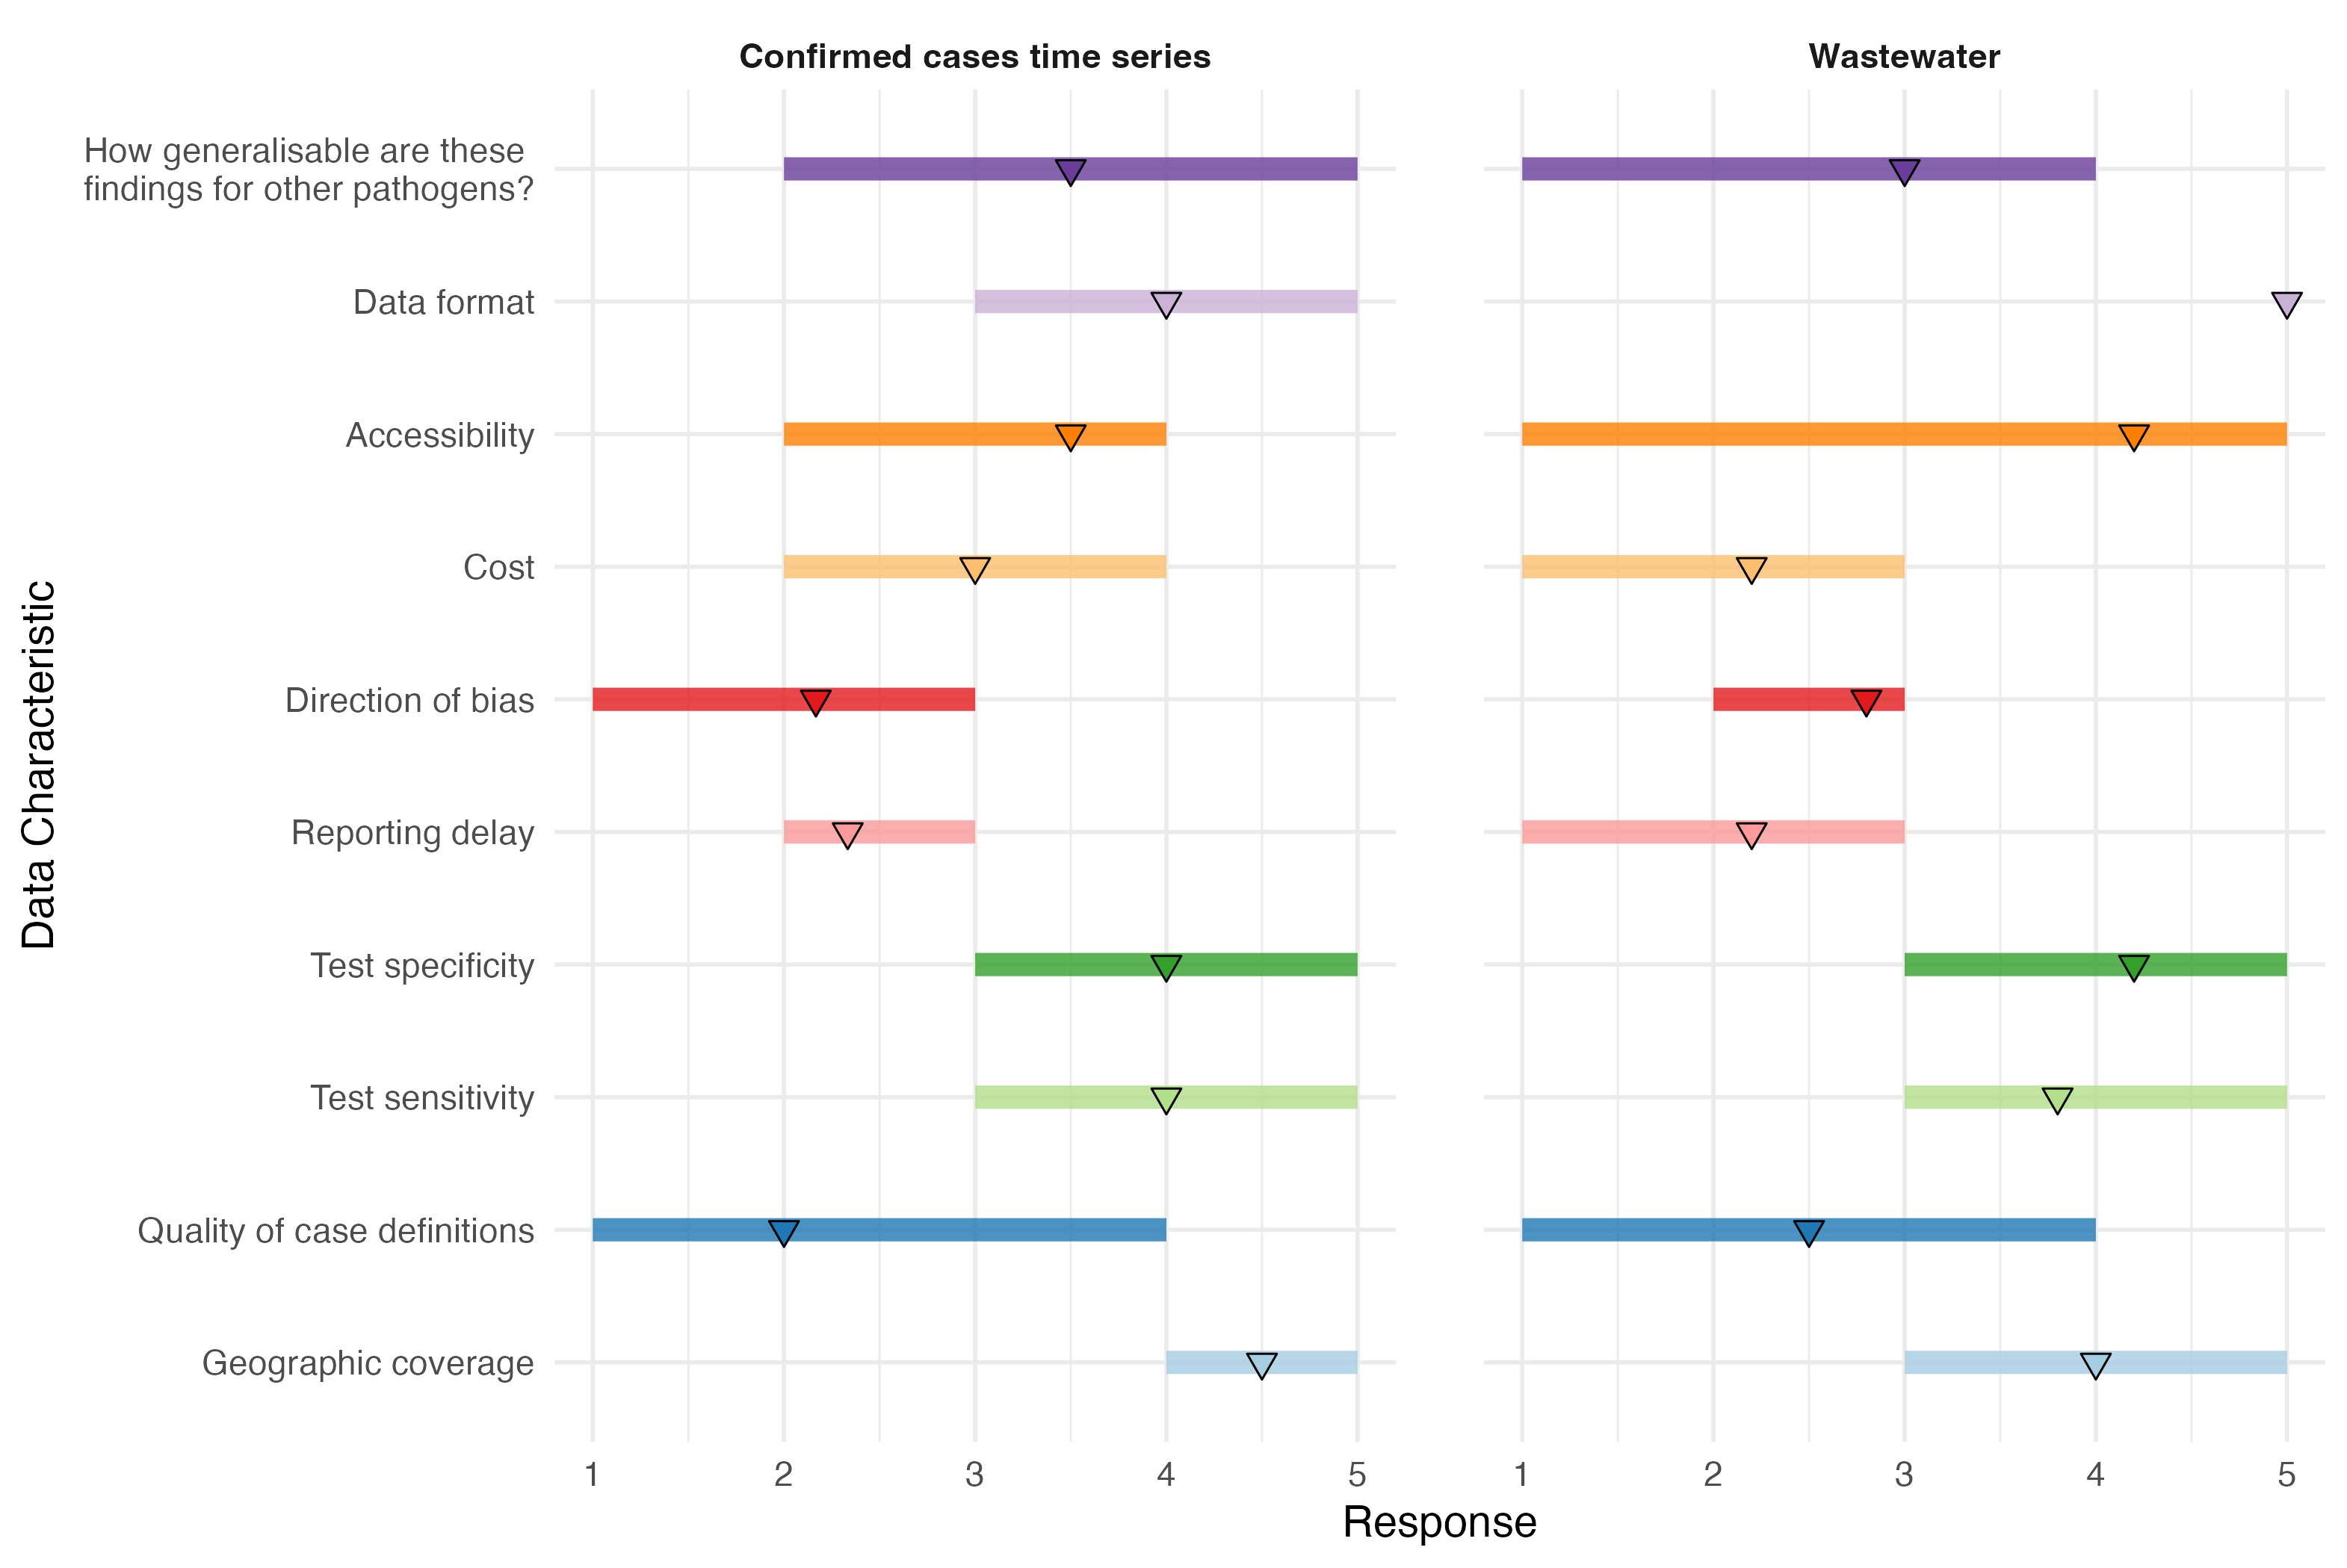
\includegraphics[width=.97\linewidth]{figures/survey_responses.png}
\centering
\caption{ Selected data characteristics from the survey, showing responses related to confirmed case time series (6 responses) and wastewater surveillance (5 responses). The y-axis represents specific data characteristics, while the x-axis indicates the response range on a 5-point scale, where 1 corresponds to a low level and 5 to a high level. The lower triangles present the average response for each data characteristic.}
\label{survey_responses}
\end{figure}



\subsection{Case Study 0: Single-Source Baseline (Cases Only)}


In this case study, we showcase the workflow and explore some of the assumptions and modelling and fitting choices underlying estimation of $R_t$ from a single time series of case incidence.

\textbf{Workflow Demonstration:}
\begin{enumerate}
    \item \textbf{Research question and target estimands:} The research question for this case study (and case studies 1 and 2) is: what is the time-varying reproduction number $R_t$ during this outbreak period?

    \item \textbf{Process DAG development:} We begin with a flexible branching process model for the number of people $N_{i,t}$ newly infected by individual $i$ on day $t$:
    \begin{equation} \label{eq:individual_level}
         N_{i,t} \sim \mathrm{Poiss} \left( Y_i R_t w_{t-T_i} \right)
    \end{equation} 
    Here, $T_i$ is the infection time of individual $i$, $Y_i$ is the relative transmission rate of individual $i$ (which may capture a combination of biological and social factors), and $w_s$ is the relative infectiousness $s$ days after infection normalised such that $\sum_{s=1}^\infty w_s=1$. This explicitly models the full transmission tree of the epidemic whilst remaining relatively parsimonious. We assume that the infectiousness profile $w_s$ does not change over time, but note that we would need to revisit this assumption if there was evidence this had changed, for example due to biological changes in the pathogen, changes in contact patterns, or case isolation measures.
    

\item \textbf{Data source selection:} Case incidence data is typically readily available with very frequent updates and relatively good timeliness (good scope and resolution), though this can depend on lab processing and reporting timelines. These factors make case data an obvious choice for trying to model time varying transmission parameters. However, case counts are an imperfect and potentially biased proxy for infection incidence, and is sensitive to testing patterns and the fraction of infections that are reported as cases (data quality issues) -- see Table \ref{tab:survey_results} and Figure \ref{survey_responses}. 


\item \textbf{Observation DAG construction:} The observation model relates the observed data (here daily case incidence) with underlying latent variables (here, daily infection incidence). 
This requires us to make assumptions about case ascertainment (what fraction of infections are detected cases), reporting delays (time between infection and a case being detected and reported), and random noise (typically used to capture other things not explicitly specified in the model).

There are at least  $2^3=8$ possible observation models to consider, which either ignore or include each of these three aspects.
We refer to these models as $O_{000}$ (for the simplest observation model not modelling any of the above) to $O_{111}$ (for the most comprehensive accounting for all three observation features). We represent the $O_{111}$ model by the following equation for the observed variable $\hat{I}_t$, representing the number of reported cases on day $t$:
\begin{equation} \label{eq:cases}
    \hat{I}_t \sim \mathrm{Poiss}\left( \sum_{s=1}^t M_{s,t}\right)
\end{equation}
where $M_{s,t}$ is the number of people infected on day $s$ and reported as a case on day $t$, given by
\begin{equation}
    M_{s,t} \sim \mathrm{TruncatedMultinomial}\left( I_s, p_c\alpha_{t-s}\right) 
\end{equation}
Here $I_s=\sum_i N_{i,s}$ is the total number of new infections on day $s$, $p_c$ is the probability an infection is reported as a case (i.e. case ascertainment rate), and $\alpha_j$ is the probability mass function of the distribution of time from infection to reporting. We choose to use the most comprehensive observation model $O_{111}$ as it is important to account of all three factors.



\item \textbf{Refine the model DAGs:} Recognising that we only have aggregate-level data on the number of reported cases and no individual-level data about the transmission tree, we realise that individual heterogeneity in transmission rates (represented by the variable $Y_i$) will not be identifiable. We therefore simplify the model by assuming that $Y_i=1$ for all individuals. With this simplification, the model for the number of new infections $I_t=\sum_i N_{i,t}$ on day $t$ reduces to
    \begin{equation} 
        I_t \sim \mathrm{Poiss}\left( R_t \sum_{s=1}^\infty I_{t-s}w_s  \right)
    \end{equation}
    This is an example of the well-known renewal process model. This is a popular model for $R_t$ estimation as it captures fundamental features of the transmission process (newly infected individuals at time $t$ transmit the pathogen to other individuals some time later), without making additional assumptions, for example about the size of the susceptible population or the strength and duration of infection-acquired immunity. This provides a simple but flexible model to which additional complexity can be added in subsequent iterations of the workflow.
    There are other valid assumptions we might wish to make depending on other workflow considerations. Here, we consider three variants of the renewal process model with differing models for the variance in daily infection incidence $I_t$:
    \begin{itemize}
    \item[$P_1$.] Deterministic model for daily infection incidence (no variance).
    \begin{equation} \label{eq:infections_P1}
        I_t = R_t \sum_{s=1}^\infty I_{t-s}w_s 
    \end{equation}
    \item[$P_2$.] Poisson-distributed daily infection incidence.
        \begin{equation} \label{eq:infections_P2}
        I_t \sim \mathrm{Poiss}\left( R_t \sum_{s=1}^\infty I_{t-s}w_s  \right)
    \end{equation}
    \item[$P_3$.] Negative binomially distributed daily infection incidence (larger variance than Poisson). 
            \begin{equation} \label{eq:infections_P3}
        I_t \sim \mathrm{NegBin}\left( R_t \sum_{s=1}^\infty I_{t-s}w_s, k  \right)
    \end{equation}
    where $k$ is the dispersion parameter. 
    \end{itemize} 
Figure \ref{fig:case_study_visual} shows the process DAGs and observation DAGs for all potential models. Here, $P_1$ is unlikely to be realistic as there will almost always be some source of random variability in daily infection incidence. The choice between $P_2$ and $P_3$ could depend on whether superspreading is known to be a major factor in the transmission dynamics. Since $P_3$ contains $P_2$ in the limiting case $k\to\infty$, we choose to use $P_3$ in this example (see Figure \ref{fig:case_study_diagram}). 


\item \textbf{Modularise the DAGs:} Here we do not need to do any modularisation as we are only dealing with a single data source.

\item \textbf{Inference and implementation choices:} Implementation requires selection of one process model, one observation model and one fitting method. The choice of fitting method depends on the analytical tractability of the combined process and observation model, computational complexity and speed of computation relative to the time available, and identifiability issues (see Section \ref{sec:fitting}). 
For our chosen combination of models ($P_3$-$O_{111}$), we recommend using NUTS but only if we approximate the discrete observation models (e.g. EpiNow2 \citep{abbott2020estimating}), or if we do not want to do this we would need to use an alternative method such as PMCMC. If a simpler, more computationally efficient fitting method were needed, we could return to the ``Refine models'' stage and select a simpler model. For the simplest model combination with no underreporting, delays or observation noise ($P_1$-$O_{000}$), we can calculate $R_t$ directly for a given choice of generation time distribution by rearranging Eq. \eqref{eq:infections_P1}. This is likely to give biased and highly noisy estimates in practice and does not provide any uncertainty quantification. For the next-simplest model ($P_2$-$O_{000}$), we can calculate an analytical posterior distribution for $R_t$  from a conjugate gamma prior, which is fast and computationally efficient. This is implemented in the widely used EpiEstim method \citep{cori2013new}. 

\item \textbf{Model specification and validation:} Model specification requires a prior for $R_t$ as well as specification of the profile of infectiousness over time $w_t$, the reporting probability $p_c$, the distribution of time from infection to reporting $\alpha_t$ and (for process model $P_3$) the dispersion coefficient $k$. The simplest approach is to take these as fixed parameters, which corresponds to an infinite-strength prior. This is unlikely to ever be appropriate but may be required for computational tractability. However, a better approach in the presence of uncertainty is to define a prior over these parameters based on domain expertise. In the case of probability distributions $w_t$ and $\alpha_t$, this could take the form of a parametric distribution assumption, e.g. a discretised gamma \citep{charniga2024best,park2024estimating} or other non-negative-integer valued distribution with specified priors for the mean and variance. 

Different modelling approaches have different strengths and limitations. For example, simple approaches are fast to implement, but ignore important factors in the data observation process. These may be useful for a quick initial estimate, but should be revisited as needed. In this case study, $R_t$ estimates may be insensitive to underreporting provided the reporting fraction is constant over the period of interest. Furthermore, any change in reporting fraction will not be identifiable from a case time series alone (if $R_t$ varies over time same time scale), so it would not be sensible to attempt to estimate this in this example. However, reporting delays can be substantial and will affect both the magnitude and timing of $R_t$ estimates. We can account for this by selecting an appropriate observation model, at the cost of needing to move to a more computationally costly fitting method. Ultimately, the most appropriate option will depend on the balance between need for timely estimates (e.g. for modelling an outbreak in real-time) and the realism of the associated assumptions. 
Finally, a common weakness of all the models outlined above is that they assume the profile of infectiousness over time is constant. Some approaches (e.g. some versions of EpiEstim, and EpiNow2 \citep{abbott2020estimating}) extend the approach to relax this assumption.
 
\item \textbf{Data integration choices:} As there is only one data source in this case study, we do not need to make any decisions about what and how to integrate multiple sources. One scenario where integration would be required where multiple groups use different methods to produce estimates of the target estimand (in this case $R_t$) based on the same data, which we then ensemble into a combined estimate \citep{maishman2022statistical,manley2024combining}. In this context, it is desirable to align the assumptions made by different models, for example about the generation time distribution or the temporal smoothness in $R_t$, to ensure that estimates from the different models are  comparable \citep{brockhaus2023why}.

 \end{enumerate}
 


\begin{figure}[htbp]
    \centering
    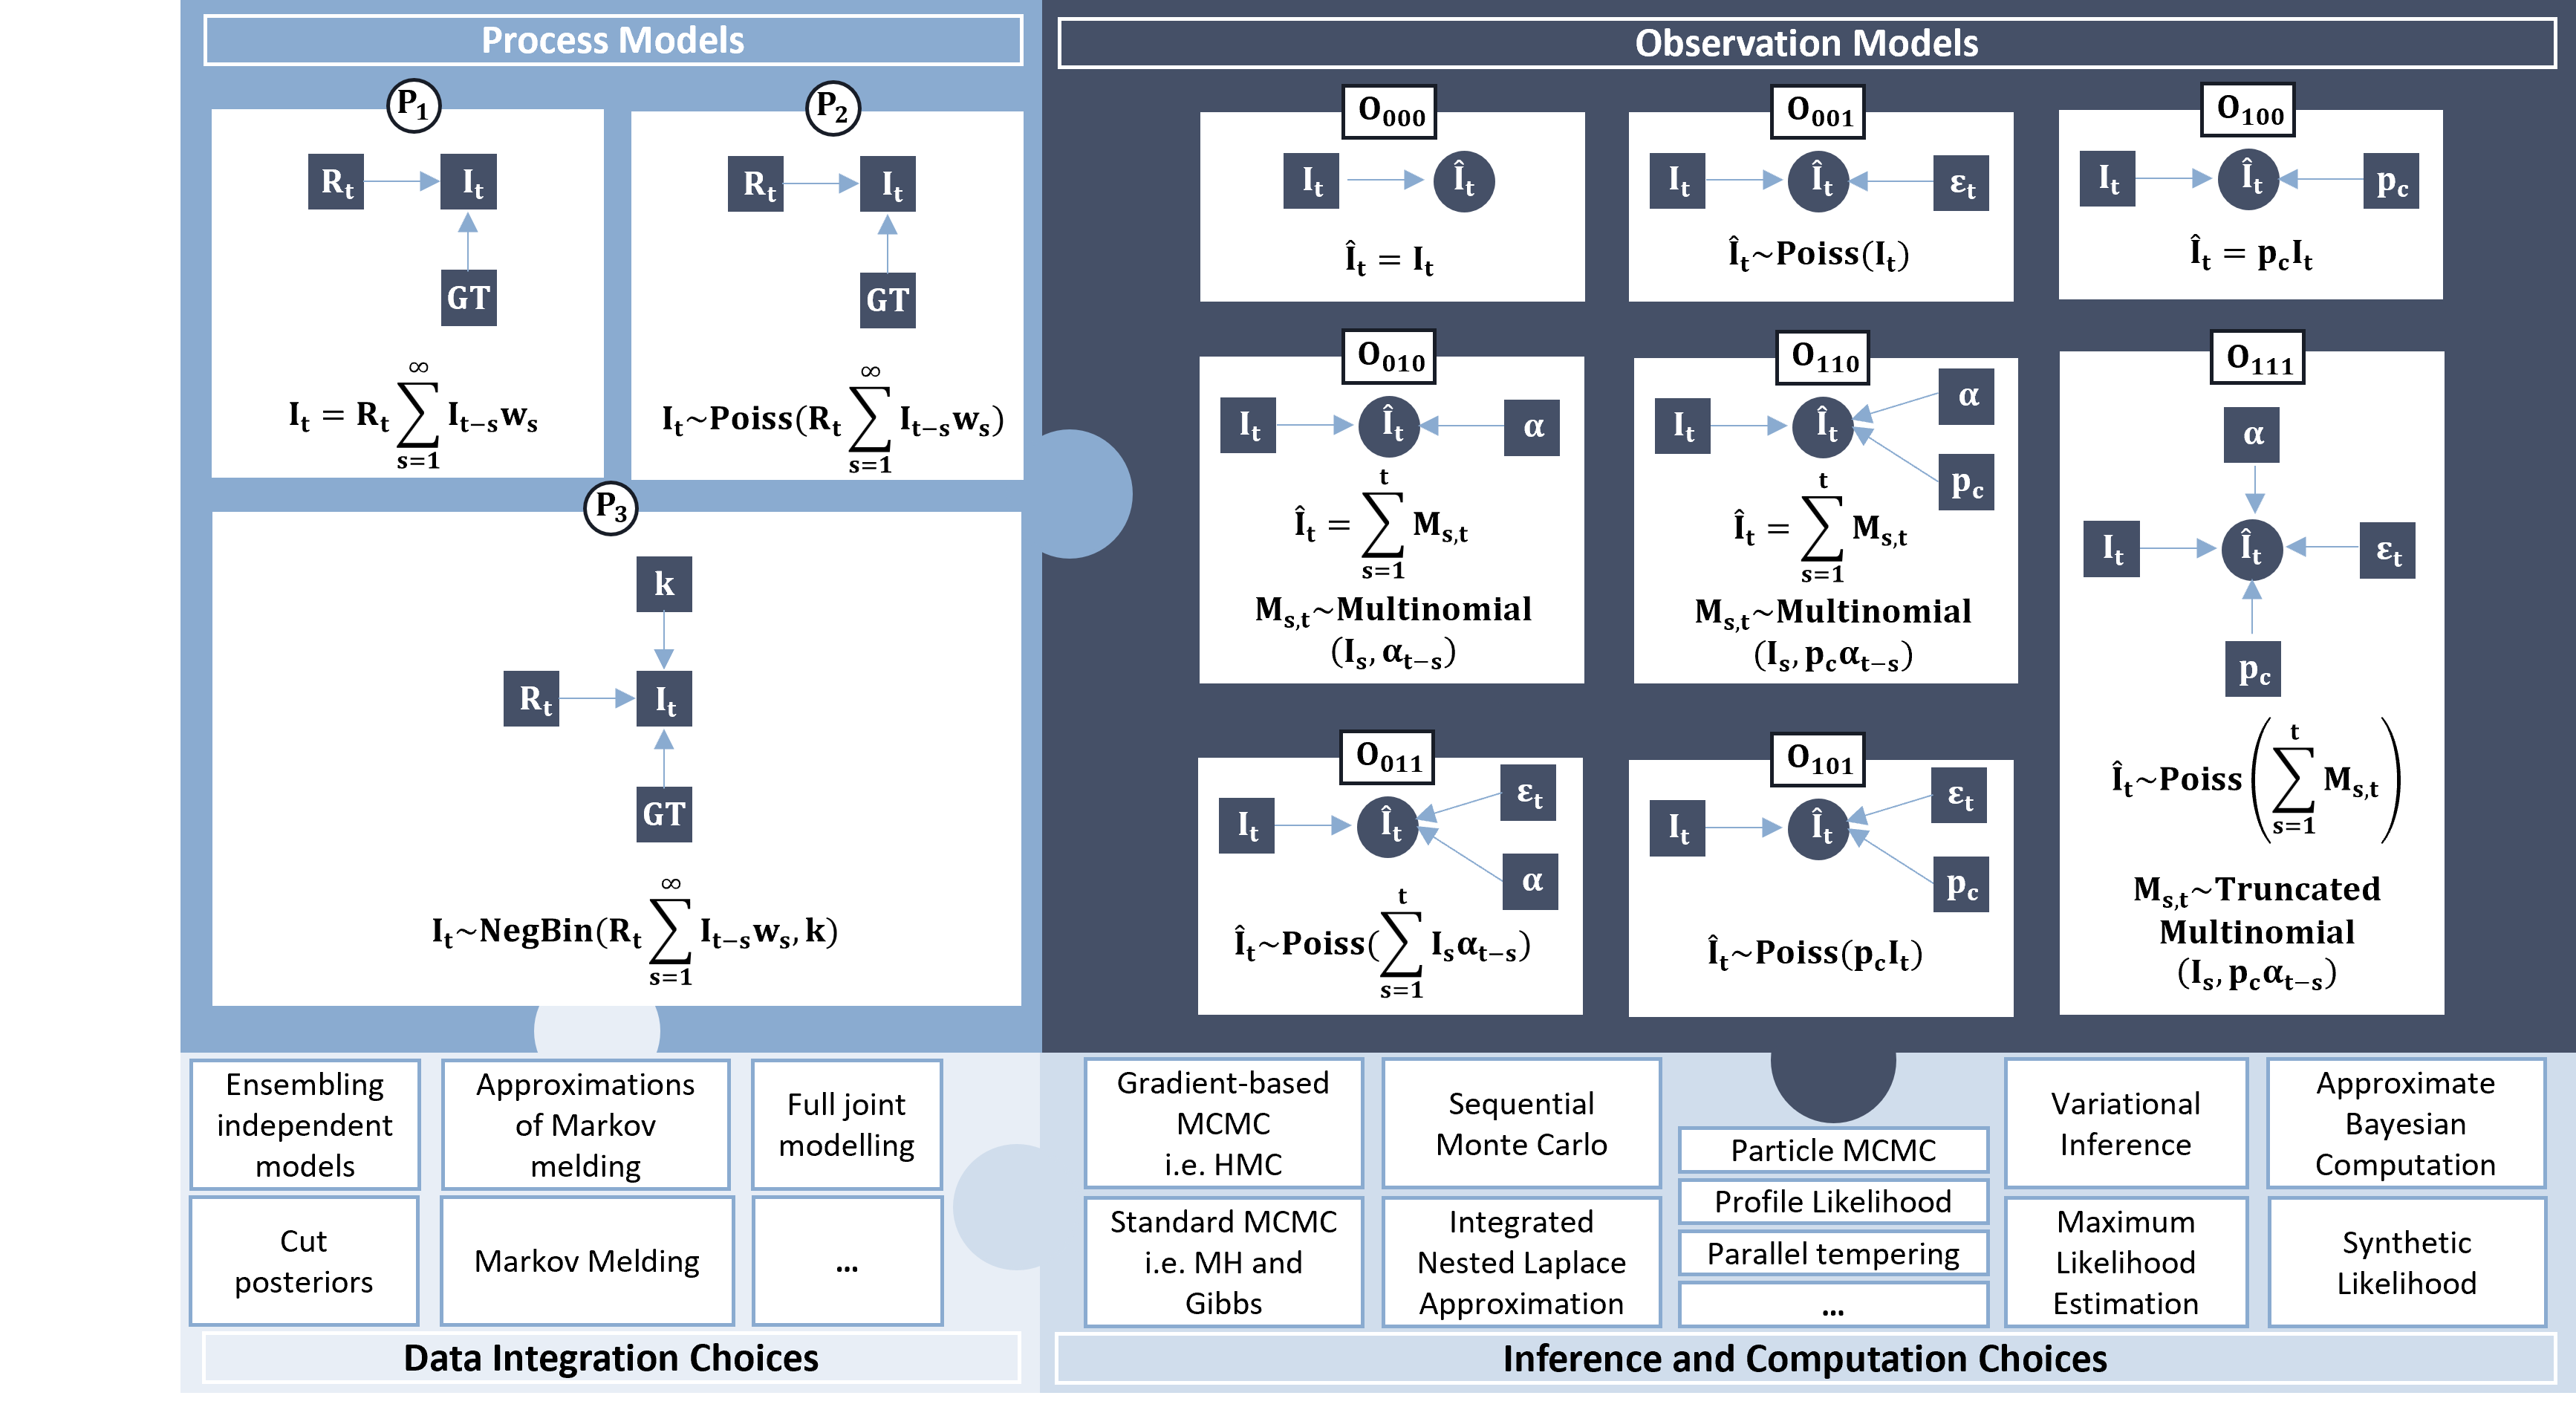
\includegraphics[width=\textwidth]{figures/case_study_puzzle_complete.png}
    \caption{\textbf{Modular representation for infectious disease modelling showing the interchangeable components of process models, observation models, integration approaches, and fitting methods.} Process models include deterministic ($P_1$), stochastic Poisson ($P_2$), and negative binomial ($P_3$) formulations relating reproduction number ($R_t$) to number of new infections ($I_t$) with generation time ($GT$) distributions. $P_3$ incorporates overdispersion parameter $k$ to caption extra-Poisson variation. Observation models range from direct observation ($O_{000}$) to complex hierarchical structures ($O_{111}$) that model the relationship between $I_t$ and (observed) case incidence through underreporting, reporting delays and measurement uncertainty. The jigsaw puzzle metaphor illustrates how different modelling components can be combined flexibly, with inference method including MCMC, VI, ABC, etc.Integration approaches span from full joint modelling to ensembling independent models, enabling researchers to select optimal combinations based on data availability and research objectives. }
    \label{fig:case_study_visual}
\end{figure}


\subsection{Case Study 1: Two-Source Integration (Cases and Deaths)}

More data sources often become available later in an outbreak. For example, early in an outbreak, surveillance data may be restricted to reported cases due to the delay from infection to development of clinically severe disease. However, data subsequently became available on other events such as hospitalisation, ICU admission or death. In this case study, we model time-varying transmission rates using two data sources: reported cases and deaths. We illustrate the process and challenges of adding an additional data stream and explore how this can improve $R_t$ estimation and reduce assumption dependence.

\begin{enumerate}
   \item \textbf{Research question and target estimands:}  In this case study, we target the same estimand as in case study 0 ($R_t$). 
   
    \item \textbf{Process DAG development:} We consider the same process DAG as in case study 0 (see Figure \ref{fig:case_study_diagram}).
        
    \item \textbf{Data source selection:} Data on deaths typically have longer delays (delay from infection to death and potentially from date of death to date of registration), but lower noise (e.g. due to ``day-of-the-week'' reporting effects), higher ascertainment, and less dependence on testing patterns than case incidence data. Combining deaths data with cases therefore has the potential to overcome some of the limitations present in each single data source. Based on the data survey (Table \ref{survey_responses}), we expect these data sources to have differing time-varying biases and so be useful for unpicking the dynamics of the underlying infection time series.
    
    \item \textbf{Observation DAG construction:} Similar to the number of reported cases defined by Eq. \eqref{eq:cases}, the number of deaths $D_t$ on day $t$ depends on the time series of infections up to day $t$, the infection-fatality ratio $p_d$, and the distribution $v_s$ of time ($s$) from infection to death. We represent this in the observation DAG (Figure \ref{fig:case_study_diagram}) and by the following convolution equation \citep{bhatt2023semi}:
    \begin{equation} \label{eq:deaths}
        D_t \sim \mathrm{Poiss}\left(p_d \sum_{s=1}^\infty I_{t-s}v_s \right)
    \end{equation}
    Other models for deaths are possible, for example using a multinomial model for the number of deaths occurring on day $s+k$ due to infections on day $s$ ($k=1,2,\ldots$). However, the Poisson model is a good approximation provided $p_d\ll 1$. 
    Eq. \eqref{eq:deaths} provides a model for the time series of daily deaths $D_t$ conditional on the time series of daily infections $I_t$ and would be coupled with one of Eqs. \eqref{eq:infections_P1}--\eqref{eq:infections_P3} that describe the dynamics of infections to produce a joint model for infections and deaths. We begin with the simplest observation model, which assumes that all deaths are recorded immediately, so the observed variable is simply $\hat{D}_t=D_t$.
    


\item \textbf{Refine the model DAGs:}       
    Similar to the different choices of observation model for cases, the observation model for deaths could include underreporting, reporting delays, and random noise. The observation model described above corresponds to $O_{000}$. However, in revisiting the data on deaths, we discovered that there was sometimes a substantial delay from date of death to date of registration \citep{seaman2022nowcasting}. If we were conducting the analysis retrospectively, we could use model $O_{000}$ for data by date of death (i.e. define $\hat{D}_t$ to be the number of deaths that occurred on day $t$). However, for a real-time analysis, this data would be incomplete and it would be important to account for the delay. Hence, we use data by date of registration (i.e. define $\hat{D}_t$ to be the number of deaths registered on day $t$) and use model $O_{010}$. This still assumes that all deaths are eventually reported with no additional observation noise (which is reasonable for jurisdictions with comprehensive death records), but accounts for the observation delay via the following equation for the number of deaths registered on day $t$:
\begin{equation}
    \hat{D}_t = \sum_{s=0}^\infty M_{s,t}
\end{equation}
where $M_{s,t}$ is the number of deaths that occurred on day $s$ and were registered on day $t$, given by
\begin{equation}
    M_{s,t} \sim \mathrm{Multinomial}\left( D_s, \beta_{t-s}\right) 
\end{equation}
and $\beta_s$ is the probability mass function for the number of days from date of death to date of registration ($s=0,1,\ldots$).

 \item \textbf{Modularise the DAGs:} The module for reported cases is the same as in case study 0. Here, we add second module for deaths (see Figure \ref{fig:case_study_diagram}).

\item \textbf{Inference and implementation choices:} As each submodel and the joint model have a differentiable likelihood, we recommend NUTS for fitting. If some of the submodels had non-differentiable likelihoods, we would recommend using NUTS on the submodels where this was possible, and PMCMC on the remaining submodels and the joint model.

\item \textbf{Model specification and validation:} In addition to the parameters from case study 0, this model requires us to specify the infection fatality ratio $p_d$, the distribution of time from infection to death $v_t$ and from date of death to date to date of registration $\beta_t$. Again, we recommend using appropriately informative priors where possible to allow for uncertainty. 


    \item \textbf{Data integration choice:} 
       Two different approaches are possible for integration: (1) a joint model including both cases and deaths with a shared latent state $R_t$ \citep{scott2020epidemia}; (2) separate models for cases and deaths, resulting in two estimates for $R_t$ to be combined via a weighted ensemble or Markov melding.
        As outlined above, we recommend fitting separate models to the two time series initially, to understand their behaviour and reveal whether they lead to consistent or conflicting estimates of $R_t$ \citep{sherratt2021exploring}. Where inconsistent results emerge from the two data sources, these could prompt us to refine the model. For example, if $R_t$ estimates show similar trends but shifted in time, assumptions about delays may be revisited (return to ``Model specification and validation step''). If $R_t$ estimates are largely consistent, but the case-based estimate shows a transient increase in $R_t$ that does not occur in the deaths-based estimate, this could indicate an increase in case ascertainment (return to ``Refine models'' step to include time-varying ascertainment). In case study 0 using data on cases alone, the case ascertainment rate (i.e. the proportion of infections that are reported as cases) was non-identifiable and had to be assumed. Including data on deaths, if the infection-fatality ratio is known, means that we could also target the case ascertainment rate for estimation using a joint model. However, this requires assumptions about the distribution of time from infection to death, demonstrating how additional data sources can shift rather than eliminate the need for modelling assumptions. 
\end{enumerate}

\subsection{Case Study 2: Three-Source Integration (Cases, Deaths and Wastewater)}

Wastewater-based epidemiology has emerged as a complementary data source to traditional disease surveillance methods \citep{keshaviah2023wastewater}. Wastewater surveillance has been applied to a range of viral pathogens including norovirus \citep{zheng2024tracking}, poliovirus \citep{whitehouse2024wastewater}, and influenza viruses \citep{zheng2023development}. During the Covid-19 pandemic, wastewater surveillance was used to support outbreak detection \citep{hewitt2022sensitivity}, situational awareness and forecasting \citep{varkila2023use,jin2024combining}, and multi-strain modelling \citep{dreifuss2025estimated}. 

\begin{enumerate}
   \item \textbf{Research question and target estimands:} In this case study, we include measurements of viral RNA/DNA concentration in wastewater samples as a third data source alongside reported cases and deaths and explore ways of handling conflicting signals between data sources and incorporating complex observation processes. The target estimand is $R_t$, as in case studies 0 and 1.
   
    \item \textbf{Process DAG development:} We consider the same process DAG as in case studies 0 and 1  (see Figure \ref{fig:case_study_diagram}).

    \item \textbf{Data source selection:} Wastewater data offers population-level information (broad scope) independent of testing biases and changes in testing rates, with moderate timeliness, but requiring environmental expertise and subject to high levels of unexplained variability. It could also be affected by unknown changes in the average shedding rate over time and has relatively poor resolution (limited spatial resolution and no information about age or other demographic variables). 

    
    \item \textbf{Observation DAG construction:} 
    Suppose that the average concentration $W_t$ of viral RNA/DNA in wastewater on day $t$ depends on the time series of infections up to day $t$ and the average amount of viral RNA/DNA that an individual sheds into wastewater $s$ days after being infected ($s=1,2,\ldots$). This can be represented in the process DAG (Figure \ref{fig:case_study_diagram}) and by the following equation for $W_t$:
    \begin{equation} \label{eq:wastewater}
        W_t = \frac{c}{N_\mathrm{pop}}\sum_{s=1}^\infty I_{t-s}u_s 
    \end{equation}
    where $c>0$ is a constant representing the average total amount of viral RNA/DNA that an infected individual sheds over the course of their infection, $N_\mathrm{pop}$ is the total population size, and $u_s$ is the average shedding rate $s$ days after infection normalised such that $\sum_{s=1}^\infty u_s=1$.  Eq. \eqref{eq:wastewater} would be coupled with one of Eqs. \eqref{eq:infections_P1}--\eqref{eq:infections_P3} for infections.
    
   Wastewater samples are typically collected at some cadence from one or more sampling sites, and the concentration of viral RNA/DNA in the samples is quantified via PCR testing. The existence of multiple sites with different catchments populations and non-contemporaneous sampling frequencies complicates the interpretation of quantitative wastewater data, which can be modelled at varying levels of complexity.   
   Suppose that measurements of the wastewater concentration $\hat{W}_{j,t}$ are taken from sampling sites $j=1,\ldots, J$ on some subset of days $t$. Similarly to \citep{watson2024jointly}, we assume that these observations are conditionally independent gamma random variables with the same mean $W_t$ and variance $b W_t^2/N_j$, where $N_j$ is the population size in the catchment for sampling site $j$ and $b$ is a variance parameter:
    \begin{equation}
        \hat{W}_{j,t} \sim \Gamma\left( W_t,  \frac{b W_t^2}{N_j} \right)
    \end{equation}

       
\item \textbf{Refine the model DAGs:}  The formulation above assumes that the different catchment areas have identical epidemic dynamics and the only difference between catchments is that those with smaller populations have higher measurement variance. This is a reasonable starting assumption if the outbreak is evenly distributed geographically. However, if different sampling sites reveal different temporal trends, this would indicate the need to refine the model to account for different epidemic dynamics in different regions. This could require revisiting the data source mapping step for an assessment of whether the catchment areas for wastewater sampling are aligned with the geographical stratification (if any) available for reported cases and deaths. More complex observation models could also incorporate other factors such as individual-level and site-level variation, catchment population dynamics, spatial heterogeneity, different sampling methods, and environmental degradation.

\item \textbf{Modularise the DAGs:} The modules for cases and deaths are the same as in case studies 0 and 1 respectively. The module for wastewater data follows the same pattern, with wastewater representing a third process downstream from the daily infection incidence.
    
    \item \textbf{Inference and implementation choices:} As before, we recommend using a gradient-based fitting method such as NUTS where possible. For real-time estimation during an outbreak, this may be impractical, in which case, we might need to consider a method such as SMC to support sequential data assimilation, provided that model parameters are known (or fixed) and the focus is primarily on state estimation.  For a joint model, the increased state-space complexity would likely require a method such as PMCMC.

    \item \textbf{Model specification and validation:} In addition to the parameters from the previous two case studies, we need to specify the average shedding rate $c$, the total population size $N_\mathrm{pop}$, the population in each sampled catchment $N_j$, and the shedding profile over time $u_t$. Wastewater data enables $R_t$ estimation independent of shifts in testing patterns, but requires assumptions about the shedding, environmental and sampling processes. Similar to the unknown case ascertainment rate in case study 0, estimates of $R_t$ will be insensitive to the value of $c$ provided it does not change over time. However, changes in the average shedding rate due to, for example, pathogenic evolution or changes in population immunity, would invalidate this simple model and require a more nuanced approach. 
    
    \item \textbf{Data integration choice:} As in case study 1, we recommend a modular approach with sequential consistency assessment to detect and resolve data source conflicts. For example, a time lag in estimates of $R_t$ from wastewater data alone relative to estimates of $R_t$ from cases alone could suggest misspecification of the shedding rate distribution $u_s$.  It is also useful to compare estimates of latent states between separate models. For example, if estimates of $I_t$ from the cases model and the wastewater model are initially consistent but start to diverge after a certain time, this could indicate that either the case ascertainment rate $p_c$ or the average shedding rate $c$ has changed. An assessment of which of these explanations is more likely might be informed by the context. For example a decrease in testing would suggest a drop in case ascertainment is likely, while a vaccine rollout might suggest that a drop in average shedding is likely due to increased immunity. 

    Once conflicts have been identified and resolved, we could combine independent estimates of $R_t$ from these models ensembling, or fit a joint model with a shared $R_t$ state. If fitting a joint model, only one of the parameters $p_c$, $p_d$ and $c$ needs to be specified, while the other two are in principle identifiable from the data. If the steps above revealed some likely time-dependence in these quantities, this could prompt us to refine the model, for example by allowing the case ascertainment rate $p_c$ or the shedding rate $c$ to be time-dependent latent states as opposed to fixed parameters \citep{watson2024jointly}. 
\end{enumerate}

\subsection{Case Study 3: Individual-Level Data (Cases and Transmission Pairs)}

In this final case study, we illustrate how we can combine different types of data (time series count data and individual-level data from contact tracing records) to enable estimation of additional quantities. 

\begin{enumerate}
   \item \textbf{Research question and target estimands:} The research question for this case study is what is the time-varying reproduction number $R_t$ and how much heterogeneity is there in individual transmission rates? The latter is captured by the additional estimand $k$, representing the dispersion in the distribution of the number of secondary cases per index case \citep{lloyd2005superspreading}. 
   
    \item \textbf{Process DAG development:} Now that we have some information on individual-level variables, as opposed to just aggregate daily counts, we can return to our original process model for the full epidemic transmission tree from case study 0, defined by Eq. \eqref{eq:individual_level} (see Figure \ref{fig:case_study_diagram}). 
    Building on the model of \citet{lloyd2005superspreading}, if $Y\sim \Gamma(1,k)$ for some dispersion parameter $k$, then the number of secondary cases caused by an individual who was infected at a given time $T_i=t$ is
     \begin{equation} \label{eq:offspring_dist}
        Z_i \ | \ (T_i=t) \sim \mathrm{NegBin}\left( \tilde{R}_{t}, k\right)
    \end{equation}   
    where $\tilde{R}_t= \sum_s R_{t+s} w_s$ is the effective reproduction number averaged over the infectious period of an individual who was infected on day $t$.
   
    \item \textbf{Data source selection:} Case studies 0, 1 and 2 only consider aggregate-level data on daily counts or wastewater measurements. This type of data typically only allows estimation of average transmission, i.e. $R_t$. In contrast, contact tracing records identify transmission pairs, which contain information about heterogeneity in transmission patterns, contingent on contact tracing system quality. The smaller the dispersion parameter $k$, the more variance would be expected in the distribution of the number of secondary infections per index case.
    
    \item \textbf{Observation DAG construction:} Suppose that, for some subset of reported cases $i$, the number of observed secondary cases $\hat{Z}_i$ associated with that index case is recorded. For simplicity, we assume that the index cases for whom these data are available are a randomly chosen subset of all reported cases, and each secondary infection independently has fixed probability $p_l$ of being linked to the index case. We assume that all linked secondary cases are associated with the correct index case (i.e. we ignore any misclassification and uncertainty about who infected whom). 

   Then the probability that an index case reported on day $\tau_i$ has $\hat{Z}_i$ linked secondary cases can be calculated by conditioning on the unobserved time of infection $T_i$:
   \begin{equation}
       P(\hat{Z}_i=z \ | \ \tau_i=t) = \sum_{s=1}^{t} F_{NB}(z; p_l\tilde{R}_s,k) P(T_i=s | \tau_i=t)
   \end{equation}
where $F_{NB}(.;\mu,k)$ is the probability mass function for a negative binomial distribution with mean $\mu$ and dispersion $k$, and $R_i$ is the reporting time for case $i$.  The conditional probability on the right-hand side of this equation can be calculated via Bayes' theorem to give
   \begin{equation} \label{eq:Zhat}
       P(\hat{Z}_i=z \ | \ \tau_i=t) = \frac{\sum_{s=1}^{t} F_{NB}(z; p_l\tilde{R}_s,k) \alpha_{t-s} I_s}{\sum_{s=1}^{t}\alpha_{t-s} I_s}  
   \end{equation}
 where $\alpha_t$ is the distribution of time from infection to reporting.

    \item \textbf{Refine the model DAGs:}  We start by assuming that the relative infectiousness profile over time $w_t$ and the distribution of time from infection to reporting $\alpha_t$ are the same for all individuals. This is a reasonable starting assumption, but it may be important to relax this in some situations, for example to model the impact of quarantine and isolation measures on individuals identified by contact tracing.

    \item \textbf{Modularise DAGs:} 
    
    \item \textbf{Inference and implementation choices:} NUTS with data augmentation for unobserved transmissions, chosen for efficient handling of discrete latent variables. Alternatively a method such as particle marginal Metropolis Hastings could be used to used to estimate the time-varying reproduction number $R_t$ and the fixed parameter $k$ hierarchically, but may be computationally slow. 

    \item \textbf{Model specification and validation:} Individual-level data enables direct overdispersion estimation without distributional assumptions but requires assumptions about the completeness of contact tracing data. This shows how data granularity can fundamentally change model structure and inference requirements. Note that the observed variable $\hat{Z}_i$ in Eq. \eqref{eq:Zhat} may not be available in real time as information about linked secondary cases takes time to collect. Furthermore, the distribution of $\hat{Z}_i$ depends on future values of the latent variable $R_t$ and this means the model is not suitable for real-time inference. If the model was found to be impractical for these reasons, it may be necessary to simplify the model by making some additional assumptions. For example, if there was a period of time in which $R_t$ was estimated to be relatively steady, the model could be simplified by assuming a constant reproduction number and estimating $k$ from contact tracing data relating to that period. 

    \item \textbf{Data integration choices:} Since the two datasets in this case study each inform different quantities (case counts inform $R_t$, data on transmission pairs inform $k$), it would not make sense to fit separate models in this example and a joint model is needed. 
\end{enumerate}


% \begin{figure}
% \centering
% (a) \\
% 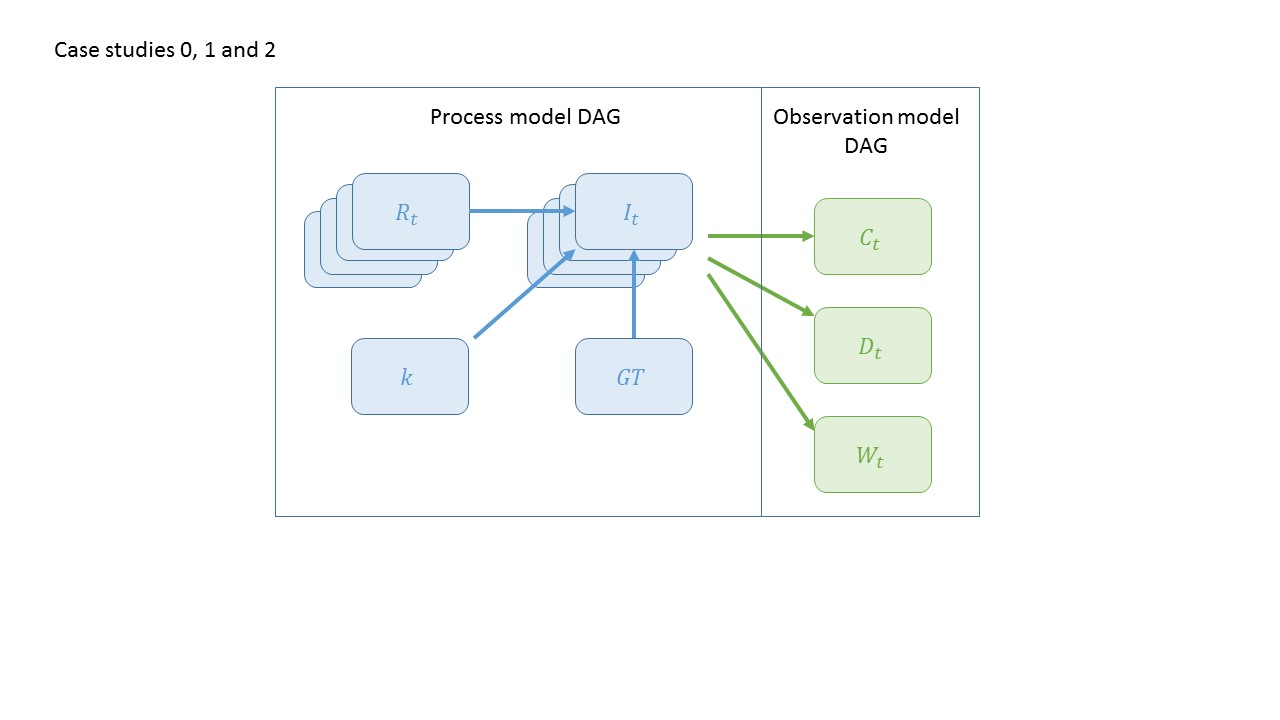
\includegraphics[width=0.75\textwidth]{figures/case_study_0_1_2.jpg}\\
% (b)\\
% 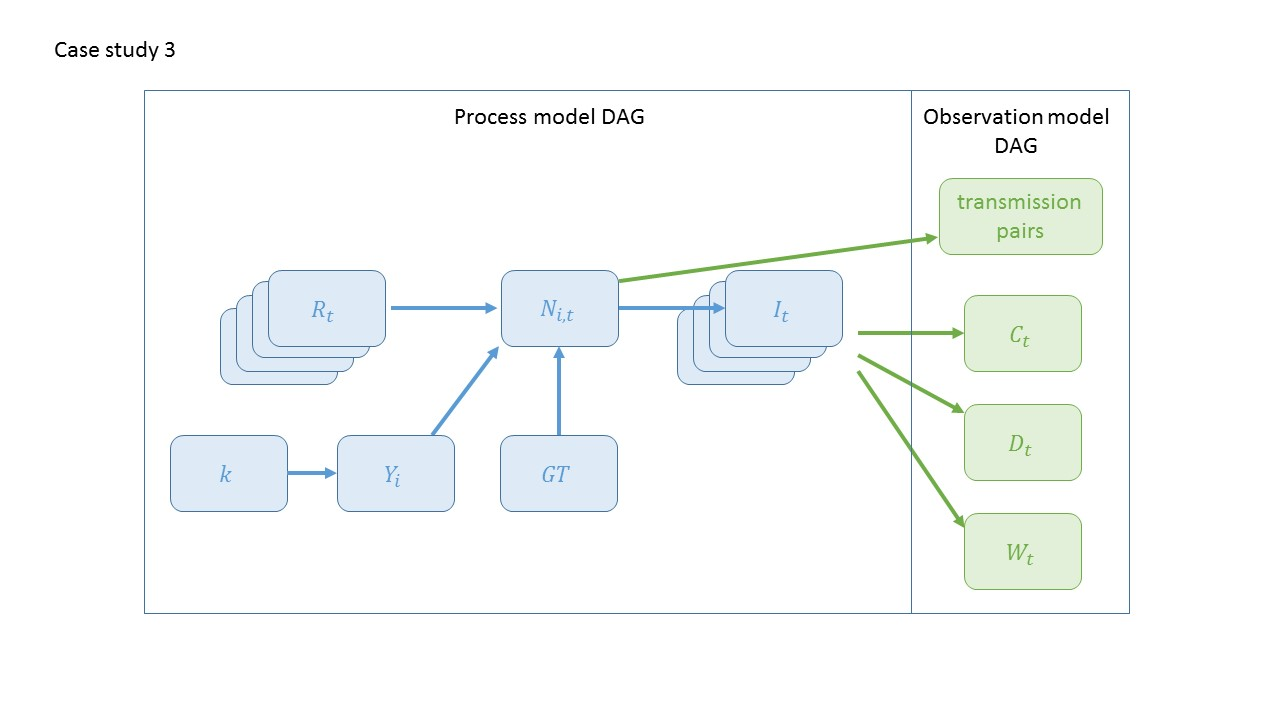
\includegraphics[width=0.75\textwidth]{figures/case_study_3.jpg}
% \label{fig:CS3_DAG}
% \caption{[Mike's attempt at DAGs for the case studies (can be made prettier later on).] Latent states in blue, observed states in green. (a) Case studies 0--2. Process model P1 is a special case where $I_t$ is a deterministic funcvtion of $R_t$ and $I_{1:t-1}$; P2 is a special case in the limit $k\to\infty$; P3 allowing the dispersion parameter $k$ to take any given value. The different observation models described in case study 0 (with or without underreporting, reporting delay, and observation noise) would affect how the expected value of the observed state $C_t$ relates to the latent states $I_{1:t}$, and the variance of the observed state $C_t$. Case studies 1 and 2 add additional observed states for deaths ($D_t$) and wasterwater observations ($W_t$) respectively. (b) Case study 3 requires more states to be inlcuded in the DAG to take account of individual heterogeneity and the impact it has on obsetved data on transmission pairs. The variable $N_{it}$ representing the number of secondary infections caused by individual $i$ on day $t$ encodes the full transmission tree. The expected value of $N_{it}$ is determined by the instantaneous reproduction number $R_t$, the relative transmission rates $Y_i$ of previously infected individuals, and their current infectiousness determined by the generation time distribution (GT). The variance in the distrubtion of $Y_i$ is determined by the dispersion parameter $k$.  }
% \end{figure}

\begin{figure}[htbp]
    \centering
    \includegraphics[width=\textwidth]{figures/case_study_diagram.drawio.pdf}
    \caption{\textbf{DAGs for Case Studies.} }
    \label{fig:case_study_diagram}
\end{figure}

\section{Discussion}

%\subsection{Summary}

We presented a framework for integrating multiple data sources in infectious disease modelling that extends established Bayesian workflow principles \citep{gelman2020bayesian}.
This workflow serves both as guidance for practitioners developing multi-source models and as a checklist for readers evaluating modelling papers.
Four case studies demonstrate this workflow using progressively more data sources for reproduction number estimation.
Each progression shows how additional data sources alter both process and observation DAGs whilst requiring new integration and fitting decisions.
We establish the baseline approach using case data to estimate $R_t$ , whilst highlighting assumptions about generation time and reporting fractions.
Adding death data eliminates some reporting assumptions but shifts dependence to infection-to-death delay assumptions and requires new integration choices.
Wastewater data provides population-level signals independent of testing biases but requires understanding viral shedding processes and likelihood-free fitting methods.
Individual-level contact tracing enables direct overdispersion estimation but leads to hierarchical process models and latent variable approaches, which can be computationally challenging.
Each case study also leads to new fitting choices and model validation strategies.
Throughout, we highlight that considering each submodel in isolation is a useful starting point for model development and validation.

%\subsection{Strengths and Limitations/Outstanding Challenges}

A key strength of our suggested workflow is the explicit separation of epidemiological process DAGs from observation DAGs, recognising that these components draw from different domains: epidemiological processes are informed by infectious disease theory, whilst observation models reflect data source characteristics and collection mechanisms.
This separation provides clarity for model development and validation.
The framework's applicability across diverse contexts, from early outbreak analysis to routine surveillance, offers flexibility for varied epidemiological questions.
In addition, our suggested data review process provides a structured approach to understanding different epidemiological data sources.
By providing explicit guidance on reporting standards, including validation procedures and code availability, we aim to improve both the development and evaluation of multi-source models.

Our suggested approach can be implemented with current tools, though doing so may require choosing between statistical rigour (resource-intensive joint models) and computational feasibility (pipeline approaches with known limitations).
The DAG-based workflow helps analysts plan for evolving data availability, but adapting models as surveillance systems change typically requires substantial work.
Teams may need to maintain multiple parallel models for different data scenarios, potentially limiting the application of this workflow in rapid responses.

Without shared infrastructure, teams typically rebuild common epidemiological processes for each application.
Current probabilistic programming frameworks provide foundations but often lack the epidemiological abstractions needed for routine use.
These implementation barriers can lead teams to adopt simpler approaches despite understanding their statistical limitations.

Workflow reporting remains inconsistent across the field, with varying levels of detail about model validation, code availability, and decision rationales.
Even when models are technically sound, incomplete reporting limits their utility for learning and adaptation.
Establishing community standards for workflow documentation would accelerate progress by enabling systematic learning from both successes and failures.

%\subsection{Comparison with Existing Literature}

 Our workflow extends Gelman et al.'s general Bayesian workflow framework \citep{gelman2020bayesian} for multi-source infectious disease modelling.
 Gelman et al. provide comprehensive model validation and criticism within a single modelling cycle with extensive guidance and practical examples.
We embed their modelling  loop within a structured workflow addressing outbreak-specific challenges: data source characterisation, integration strategies, and workflow iteration as outbreaks evolve. 
Whilst we don't give fully implemented examples, due to length and time constraints we do provide additional domain-specific guidance for surveillance data quality, reporting biases, and epidemiological process representation not covered in general statistical workflows.
 
Recent work has made progress towards structured infectious disease modelling workflows, though implementation remains incomplete.
For example, \citet{bouman2024bayesian} systematically compared modelling choices for SARS-CoV-2 transmission and provided an open-source implementation through their HETTMO package.
However, their approach, while methodologically sound, lacks the structured workflow guidance needed for broader application.
Key workflow elements such as prior predictive checks, systematic model criticism, and clear decision frameworks are absent.
Their work highlights the gap between implementing models and following robust and reproducible workflow practices.
In contrast, our framework provides explicit structured guidance through each workflow stage, with case studies demonstrating not just model implementation but the decision process itself.

%\subsection{Future work}

Future progress requires infrastructure that bridges the gap between methodological best practice and implementation.
Whilst this paper provides a schematic workflow, practical tutorials demonstrating actual implementation would provide essential guidance for practitioners.
However, such tutorials and tools require advances in software composability, where self-contained components can be combined to build complex models.
This would enable domain experts to contribute specialised components without rebuilding core functionality and make all steps of our proposed workflow easier to implement.
Improved tooling for Markov melding and cut fitting approaches would facilitate modular integration, allowing teams to combine submodels without full joint specification or specialist knowledge.
Computational scalability remains an area where more work is needed, particularly for joint analysis of individual-level genomic data with population surveillance.
Recent advances in machine learning-augmented fitting methods show promise, with neural network-based summary statistic construction \citep{raynal2019abc} and deep learning phylodynamic methods \citep{voznica2022deep} providing alternatives to traditional likelihood evaluation.

%\section{Conclusions}

Infectious disease modelling workflows benefit from systematic approaches that can adapt to multiple data sources and evolving outbreak contexts.
We have presented workflow best practices that provide practical guidance for navigating trade-offs between information gain, computational complexity, and interpretability.
Our workflow extends established Bayesian principles through structured steps from data characterisation to model validation, supported by structured evaluation of data source characteristics and multiple case studies.
The modular approach we advocate enables practitioners to build complexity incrementally whilst maintaining transparency about modelling assumptions and integration choices.
We recommend that the infectious disease modelling community adopt these workflow best practices for both model development and evaluation.
Readers can use our framework as a systematic checklist when evaluating modelling papers to assess whether workflow choices are appropriate and transparent.
Practitioners should implement these approaches across all infectious disease modelling contexts, with particular value during rapidly evolving outbreaks where research questions shift and new data sources emerge.
Establishing community standards around systematic workflow practices will improve both methodological rigour and practical implementation across the field.

\section{Acknowledgements}

We thank the organisers and participants of the workshop ``Analysis and modelling for the design of future epidemic surveillance systems'' (CIRM, Marseille, 28 April–2 May 2025) for valuable discussions and feedback that helped shape this work.
All workshop participants provided useful discussion and feedback.
We thank Poppy the dog for making sure to ask the important questions.

\bibliographystyle{plainnat}
\bibliography{references,zotero-references}


\end{document}
 